\documentclass[conference]{IEEEtran}
\IEEEoverridecommandlockouts
\usepackage{cite}
\usepackage{amsmath,amssymb,amsfonts}
\usepackage{graphicx}
\usepackage{booktabs}
\usepackage{multirow}
\usepackage{xcolor}
\usepackage{url}
\usepackage[hidelinks]{hyperref}
\graphicspath{{../../figures/}}
% generated by scripts/make_p2_numbers.py -- do not edit
\newcommand{\pMaeHAFifteen}{4.19}
\newcommand{\pRmseHAFifteen}{7.86}
\newcommand{\pMapeHAFifteen}{13.1}
\newcommand{\pMaeHAThirty}{4.19}
\newcommand{\pRmseHAThirty}{7.86}
\newcommand{\pMapeHAThirty}{13.1}
\newcommand{\pMaeHASixty}{4.19}
\newcommand{\pRmseHASixty}{7.86}
\newcommand{\pMapeHASixty}{13.1}
\newcommand{\pMaeHAAvg}{4.19}
\newcommand{\pRmseHAAvg}{7.86}
\newcommand{\pMapeHAAvg}{13.1}
\newcommand{\pMaePersFifteen}{3.49}
\newcommand{\pRmsePersFifteen}{6.38}
\newcommand{\pMapePersFifteen}{8.6}
\newcommand{\pMaePersThirty}{4.18}
\newcommand{\pRmsePersThirty}{8.00}
\newcommand{\pMapePersThirty}{10.8}
\newcommand{\pMaePersSixty}{5.33}
\newcommand{\pRmsePersSixty}{10.27}
\newcommand{\pMapePersSixty}{14.4}
\newcommand{\pMaePersAvg}{4.33}
\newcommand{\pRmsePersAvg}{8.37}
\newcommand{\pMapePersAvg}{11.3}
\newcommand{\pMaeRidgeFifteen}{3.23}
\newcommand{\pRmseRidgeFifteen}{5.75}
\newcommand{\pMapeRidgeFifteen}{8.8}
\newcommand{\pMaeRidgeThirty}{3.92}
\newcommand{\pRmseRidgeThirty}{6.98}
\newcommand{\pMapeRidgeThirty}{11.4}
\newcommand{\pMaeRidgeSixty}{4.96}
\newcommand{\pRmseRidgeSixty}{8.44}
\newcommand{\pMapeRidgeSixty}{15.1}
\newcommand{\pMaeRidgeAvg}{4.04}
\newcommand{\pRmseRidgeAvg}{7.14}
\newcommand{\pMapeRidgeAvg}{11.8}
\newcommand{\pMaeXGBlFifteen}{2.99}
\newcommand{\pRmseXGBlFifteen}{5.52}
\newcommand{\pMapeXGBlFifteen}{8.2}
\newcommand{\pMaeXGBlThirty}{3.44}
\newcommand{\pRmseXGBlThirty}{6.45}
\newcommand{\pMapeXGBlThirty}{10.0}
\newcommand{\pMaeXGBlSixty}{3.85}
\newcommand{\pRmseXGBlSixty}{7.26}
\newcommand{\pMapeXGBlSixty}{11.6}
\newcommand{\pMaeXGBlAvg}{3.43}
\newcommand{\pRmseXGBlAvg}{6.45}
\newcommand{\pMapeXGBlAvg}{9.9}
\newcommand{\pMaeXGBsFifteen}{2.87}
\newcommand{\pRmseXGBsFifteen}{5.18}
\newcommand{\pMapeXGBsFifteen}{7.6}
\newcommand{\pMaeXGBsThirty}{3.32}
\newcommand{\pRmseXGBsThirty}{6.16}
\newcommand{\pMapeXGBsThirty}{9.4}
\newcommand{\pMaeXGBsSixty}{3.78}
\newcommand{\pRmseXGBsSixty}{7.07}
\newcommand{\pMapeXGBsSixty}{11.2}
\newcommand{\pMaeXGBsAvg}{3.32}
\newcommand{\pRmseXGBsAvg}{6.18}
\newcommand{\pMapeXGBsAvg}{9.4}
\newcommand{\pMaeRFlFifteen}{2.97}
\newcommand{\pRmseRFlFifteen}{5.44}
\newcommand{\pMapeRFlFifteen}{8.2}
\newcommand{\pMaeRFlThirty}{3.42}
\newcommand{\pRmseRFlThirty}{6.38}
\newcommand{\pMapeRFlThirty}{9.9}
\newcommand{\pMaeRFlSixty}{3.87}
\newcommand{\pRmseRFlSixty}{7.25}
\newcommand{\pMapeRFlSixty}{11.7}
\newcommand{\pMaeRFlAvg}{3.42}
\newcommand{\pRmseRFlAvg}{6.40}
\newcommand{\pMapeRFlAvg}{9.9}
\newcommand{\pMaeRFsFifteen}{2.87}
\newcommand{\pRmseRFsFifteen}{5.16}
\newcommand{\pMapeRFsFifteen}{7.7}
\newcommand{\pMaeRFsThirty}{3.31}
\newcommand{\pRmseRFsThirty}{6.09}
\newcommand{\pMapeRFsThirty}{9.4}
\newcommand{\pMaeRFsSixty}{3.81}
\newcommand{\pRmseRFsSixty}{7.06}
\newcommand{\pMapeRFsSixty}{11.3}
\newcommand{\pMaeRFsAvg}{3.33}
\newcommand{\pRmseRFsAvg}{6.15}
\newcommand{\pMapeRFsAvg}{9.4}
\newcommand{\pMaeGCNFifteen}{2.88}
\newcommand{\pRmseGCNFifteen}{5.51}
\newcommand{\pMapeGCNFifteen}{7.7}
\newcommand{\pMaeGCNThirty}{3.24}
\newcommand{\pRmseGCNThirty}{6.41}
\newcommand{\pMapeGCNThirty}{9.1}
\newcommand{\pMaeGCNSixty}{3.66}
\newcommand{\pRmseGCNSixty}{7.44}
\newcommand{\pMapeGCNSixty}{10.9}
\newcommand{\pMaeGCNAvg}{3.26}
\newcommand{\pRmseGCNAvg}{6.50}
\newcommand{\pMapeGCNAvg}{9.2}
\newcommand{\pMaeGRUFifteen}{2.91}
\newcommand{\pRmseGRUFifteen}{5.71}
\newcommand{\pMapeGRUFifteen}{8.0}
\newcommand{\pMaeGRUThirty}{3.31}
\newcommand{\pRmseGRUThirty}{6.68}
\newcommand{\pMapeGRUThirty}{9.6}
\newcommand{\pMaeGRUSixty}{3.71}
\newcommand{\pRmseGRUSixty}{7.69}
\newcommand{\pMapeGRUSixty}{11.4}
\newcommand{\pMaeGRUAvg}{3.31}
\newcommand{\pRmseGRUAvg}{6.74}
\newcommand{\pMapeGRUAvg}{9.7}
\newcommand{\pMaeHybFifteen}{2.80}
\newcommand{\pRmseHybFifteen}{5.20}
\newcommand{\pMapeHybFifteen}{7.4}
\newcommand{\pMaeHybThirty}{3.23}
\newcommand{\pRmseHybThirty}{6.19}
\newcommand{\pMapeHybThirty}{9.1}
\newcommand{\pMaeHybSixty}{3.68}
\newcommand{\pRmseHybSixty}{7.15}
\newcommand{\pMapeHybSixty}{11.0}
\newcommand{\pMaeHybAvg}{3.23}
\newcommand{\pRmseHybAvg}{6.23}
\newcommand{\pMapeHybAvg}{9.2}
\newcommand{\pMaeHybNoFifteen}{2.81}
\newcommand{\pRmseHybNoFifteen}{5.20}
\newcommand{\pMapeHybNoFifteen}{7.5}
\newcommand{\pMaeHybNoThirty}{3.24}
\newcommand{\pRmseHybNoThirty}{6.19}
\newcommand{\pMapeHybNoThirty}{9.2}
\newcommand{\pMaeHybNoSixty}{3.70}
\newcommand{\pRmseHybNoSixty}{7.15}
\newcommand{\pMapeHybNoSixty}{11.2}
\newcommand{\pMaeHybNoAvg}{3.25}
\newcommand{\pRmseHybNoAvg}{6.23}
\newcommand{\pMapeHybNoAvg}{9.3}
\newcommand{\pMaeOneHopFifteen}{3.00}
\newcommand{\pRmseOneHopFifteen}{5.79}
\newcommand{\pMapeOneHopFifteen}{8.6}
\newcommand{\pMaeOneHopThirty}{3.44}
\newcommand{\pRmseOneHopThirty}{6.87}
\newcommand{\pMapeOneHopThirty}{10.4}
\newcommand{\pMaeOneHopSixty}{4.09}
\newcommand{\pRmseOneHopSixty}{8.26}
\newcommand{\pMapeOneHopSixty}{12.9}
\newcommand{\pMaeOneHopAvg}{3.51}
\newcommand{\pRmseOneHopAvg}{7.05}
\newcommand{\pMapeOneHopAvg}{10.6}
\newcommand{\pMaeThreeHopFifteen}{2.98}
\newcommand{\pRmseThreeHopFifteen}{5.69}
\newcommand{\pMapeThreeHopFifteen}{8.2}
\newcommand{\pMaeThreeHopThirty}{3.39}
\newcommand{\pRmseThreeHopThirty}{6.69}
\newcommand{\pMapeThreeHopThirty}{9.8}
\newcommand{\pMaeThreeHopSixty}{3.97}
\newcommand{\pRmseThreeHopSixty}{7.99}
\newcommand{\pMapeThreeHopSixty}{12.3}
\newcommand{\pMaeThreeHopAvg}{3.45}
\newcommand{\pRmseThreeHopAvg}{6.86}
\newcommand{\pMapeThreeHopAvg}{10.1}
\newcommand{\pMaeLWRFifteen}{2.88}
\newcommand{\pRmseLWRFifteen}{5.53}
\newcommand{\pMapeLWRFifteen}{7.9}
\newcommand{\pMaeLWRThirty}{3.25}
\newcommand{\pRmseLWRThirty}{6.46}
\newcommand{\pMapeLWRThirty}{9.4}
\newcommand{\pMaeLWRSixty}{3.68}
\newcommand{\pRmseLWRSixty}{7.50}
\newcommand{\pMapeLWRSixty}{11.2}
\newcommand{\pMaeLWRAvg}{3.27}
\newcommand{\pRmseLWRAvg}{6.54}
\newcommand{\pMapeLWRAvg}{9.5}
\newcommand{\pMaeNoDropFifteen}{2.95}
\newcommand{\pRmseNoDropFifteen}{5.66}
\newcommand{\pMapeNoDropFifteen}{8.2}
\newcommand{\pMaeNoDropThirty}{3.37}
\newcommand{\pRmseNoDropThirty}{6.69}
\newcommand{\pMapeNoDropThirty}{10.0}
\newcommand{\pMaeNoDropSixty}{3.93}
\newcommand{\pRmseNoDropSixty}{7.91}
\newcommand{\pMapeNoDropSixty}{12.4}
\newcommand{\pMaeNoDropAvg}{3.42}
\newcommand{\pRmseNoDropAvg}{6.81}
\newcommand{\pMapeNoDropAvg}{10.2}
\newcommand{\pMaeRandFifteen}{2.99}
\newcommand{\pRmseRandFifteen}{5.77}
\newcommand{\pMapeRandFifteen}{8.3}
\newcommand{\pMaeRandThirty}{3.44}
\newcommand{\pRmseRandThirty}{6.85}
\newcommand{\pMapeRandThirty}{10.0}
\newcommand{\pMaeRandSixty}{4.08}
\newcommand{\pRmseRandSixty}{8.20}
\newcommand{\pMapeRandSixty}{12.6}
\newcommand{\pMaeRandAvg}{3.50}
\newcommand{\pRmseRandAvg}{7.01}
\newcommand{\pMapeRandAvg}{10.3}
\newcommand{\pMaeSeedAFifteen}{2.97}
\newcommand{\pRmseSeedAFifteen}{5.67}
\newcommand{\pMapeSeedAFifteen}{8.3}
\newcommand{\pMaeSeedAThirty}{3.41}
\newcommand{\pRmseSeedAThirty}{6.72}
\newcommand{\pMapeSeedAThirty}{10.1}
\newcommand{\pMaeSeedASixty}{4.01}
\newcommand{\pRmseSeedASixty}{8.06}
\newcommand{\pMapeSeedASixty}{12.7}
\newcommand{\pMaeSeedAAvg}{3.46}
\newcommand{\pRmseSeedAAvg}{6.89}
\newcommand{\pMapeSeedAAvg}{10.4}
\newcommand{\pMaeSeedBFifteen}{2.94}
\newcommand{\pRmseSeedBFifteen}{5.65}
\newcommand{\pMapeSeedBFifteen}{8.2}
\newcommand{\pMaeSeedBThirty}{3.37}
\newcommand{\pRmseSeedBThirty}{6.70}
\newcommand{\pMapeSeedBThirty}{9.9}
\newcommand{\pMaeSeedBSixty}{3.97}
\newcommand{\pRmseSeedBSixty}{7.98}
\newcommand{\pMapeSeedBSixty}{12.4}
\newcommand{\pMaeSeedBAvg}{3.43}
\newcommand{\pRmseSeedBAvg}{6.84}
\newcommand{\pMapeSeedBAvg}{10.2}
\newcommand{\pMaeShortFifteen}{3.00}
\newcommand{\pRmseShortFifteen}{5.77}
\newcommand{\pMapeShortFifteen}{8.6}
\newcommand{\pMaeShortThirty}{3.44}
\newcommand{\pRmseShortThirty}{6.84}
\newcommand{\pMapeShortThirty}{10.4}
\newcommand{\pMaeShortSixty}{4.08}
\newcommand{\pRmseShortSixty}{8.22}
\newcommand{\pMapeShortSixty}{13.0}
\newcommand{\pMaeShortAvg}{3.51}
\newcommand{\pRmseShortAvg}{7.02}
\newcommand{\pMapeShortAvg}{10.7}
\newcommand{\pMaeUndirFifteen}{2.98}
\newcommand{\pRmseUndirFifteen}{5.74}
\newcommand{\pMapeUndirFifteen}{8.5}
\newcommand{\pMaeUndirThirty}{3.41}
\newcommand{\pRmseUndirThirty}{6.78}
\newcommand{\pMapeUndirThirty}{10.2}
\newcommand{\pMaeUndirSixty}{4.03}
\newcommand{\pRmseUndirSixty}{8.12}
\newcommand{\pMapeUndirSixty}{12.7}
\newcommand{\pMaeUndirAvg}{3.48}
\newcommand{\pRmseUndirAvg}{6.95}
\newcommand{\pMapeUndirAvg}{10.5}
\newcommand{\pMaeZeroFifteen}{3.03}
\newcommand{\pRmseZeroFifteen}{5.89}
\newcommand{\pMapeZeroFifteen}{8.6}
\newcommand{\pMaeZeroThirty}{3.46}
\newcommand{\pRmseZeroThirty}{6.88}
\newcommand{\pMapeZeroThirty}{10.1}
\newcommand{\pMaeZeroSixty}{4.09}
\newcommand{\pRmseZeroSixty}{8.22}
\newcommand{\pMapeZeroSixty}{12.7}
\newcommand{\pMaeZeroAvg}{3.53}
\newcommand{\pRmseZeroAvg}{7.06}
\newcommand{\pMapeZeroAvg}{10.5}
\newcommand{\pMaeGATFifteen}{2.88}
\newcommand{\pRmseGATFifteen}{5.52}
\newcommand{\pMapeGATFifteen}{7.9}
\newcommand{\pMaeGATThirty}{3.26}
\newcommand{\pRmseGATThirty}{6.46}
\newcommand{\pMapeGATThirty}{9.5}
\newcommand{\pMaeGATSixty}{3.68}
\newcommand{\pRmseGATSixty}{7.52}
\newcommand{\pMapeGATSixty}{11.3}
\newcommand{\pMaeGATAvg}{3.27}
\newcommand{\pRmseGATAvg}{6.55}
\newcommand{\pMapeGATAvg}{9.5}
\newcommand{\pValHAFifteen}{4.32}
\newcommand{\pValHAThirty}{4.32}
\newcommand{\pValHASixty}{4.30}
\newcommand{\pValHAAvg}{4.31}
\newcommand{\pValPersFifteen}{3.21}
\newcommand{\pValPersThirty}{3.80}
\newcommand{\pValPersSixty}{4.75}
\newcommand{\pValPersAvg}{3.92}
\newcommand{\pValRidgeFifteen}{3.10}
\newcommand{\pValRidgeThirty}{3.82}
\newcommand{\pValRidgeSixty}{4.87}
\newcommand{\pValRidgeAvg}{3.93}
\newcommand{\pValXGBlFifteen}{2.85}
\newcommand{\pValXGBlThirty}{3.31}
\newcommand{\pValXGBlSixty}{3.75}
\newcommand{\pValXGBlAvg}{3.30}
\newcommand{\pValXGBsFifteen}{2.70}
\newcommand{\pValXGBsThirty}{3.16}
\newcommand{\pValXGBsSixty}{3.63}
\newcommand{\pValXGBsAvg}{3.16}
\newcommand{\pValRFlFifteen}{2.86}
\newcommand{\pValRFlThirty}{3.32}
\newcommand{\pValRFlSixty}{3.79}
\newcommand{\pValRFlAvg}{3.32}
\newcommand{\pValRFsFifteen}{2.73}
\newcommand{\pValRFsThirty}{3.16}
\newcommand{\pValRFsSixty}{3.69}
\newcommand{\pValRFsAvg}{3.19}
\newcommand{\pValGCNFifteen}{2.65}
\newcommand{\pValGCNThirty}{2.98}
\newcommand{\pValGCNSixty}{3.38}
\newcommand{\pValGCNAvg}{3.00}
\newcommand{\pValGRUFifteen}{2.68}
\newcommand{\pValGRUThirty}{3.05}
\newcommand{\pValGRUSixty}{3.45}
\newcommand{\pValGRUAvg}{3.06}
\newcommand{\pValHybFifteen}{2.60}
\newcommand{\pValHybThirty}{3.01}
\newcommand{\pValHybSixty}{3.45}
\newcommand{\pValHybAvg}{3.02}
\newcommand{\pValHybNoFifteen}{2.61}
\newcommand{\pValHybNoThirty}{3.03}
\newcommand{\pValHybNoSixty}{3.48}
\newcommand{\pValHybNoAvg}{3.04}
\newcommand{\pValOneHopFifteen}{2.76}
\newcommand{\pValOneHopThirty}{3.15}
\newcommand{\pValOneHopSixty}{3.70}
\newcommand{\pValOneHopAvg}{3.20}
\newcommand{\pValThreeHopFifteen}{2.75}
\newcommand{\pValThreeHopThirty}{3.11}
\newcommand{\pValThreeHopSixty}{3.63}
\newcommand{\pValThreeHopAvg}{3.16}
\newcommand{\pValLWRFifteen}{2.65}
\newcommand{\pValLWRThirty}{2.99}
\newcommand{\pValLWRSixty}{3.40}
\newcommand{\pValLWRAvg}{3.01}
\newcommand{\pValNoDropFifteen}{2.72}
\newcommand{\pValNoDropThirty}{3.08}
\newcommand{\pValNoDropSixty}{3.57}
\newcommand{\pValNoDropAvg}{3.13}
\newcommand{\pValRandFifteen}{2.77}
\newcommand{\pValRandThirty}{3.16}
\newcommand{\pValRandSixty}{3.72}
\newcommand{\pValRandAvg}{3.22}
\newcommand{\pValSeedAFifteen}{2.74}
\newcommand{\pValSeedAThirty}{3.12}
\newcommand{\pValSeedASixty}{3.64}
\newcommand{\pValSeedAAvg}{3.17}
\newcommand{\pValSeedBFifteen}{2.71}
\newcommand{\pValSeedBThirty}{3.08}
\newcommand{\pValSeedBSixty}{3.62}
\newcommand{\pValSeedBAvg}{3.14}
\newcommand{\pValShortFifteen}{2.76}
\newcommand{\pValShortThirty}{3.14}
\newcommand{\pValShortSixty}{3.69}
\newcommand{\pValShortAvg}{3.20}
\newcommand{\pValUndirFifteen}{2.74}
\newcommand{\pValUndirThirty}{3.12}
\newcommand{\pValUndirSixty}{3.66}
\newcommand{\pValUndirAvg}{3.17}
\newcommand{\pValZeroFifteen}{2.82}
\newcommand{\pValZeroThirty}{3.17}
\newcommand{\pValZeroSixty}{3.70}
\newcommand{\pValZeroAvg}{3.23}
\newcommand{\pValGATFifteen}{2.65}
\newcommand{\pValGATThirty}{3.00}
\newcommand{\pValGATSixty}{3.39}
\newcommand{\pValGATAvg}{3.01}
\newcommand{\pPeakHAFifteen}{6.53}
\newcommand{\pOffHAFifteen}{3.60}
\newcommand{\pPeakHAThirty}{6.53}
\newcommand{\pOffHAThirty}{3.60}
\newcommand{\pPeakHASixty}{6.53}
\newcommand{\pOffHASixty}{3.60}
\newcommand{\pPeakPersFifteen}{4.56}
\newcommand{\pOffPersFifteen}{3.21}
\newcommand{\pPeakPersThirty}{5.82}
\newcommand{\pOffPersThirty}{3.77}
\newcommand{\pPeakPersSixty}{7.79}
\newcommand{\pOffPersSixty}{4.71}
\newcommand{\pPeakRidgeFifteen}{4.53}
\newcommand{\pOffRidgeFifteen}{2.90}
\newcommand{\pPeakRidgeThirty}{5.81}
\newcommand{\pOffRidgeThirty}{3.45}
\newcommand{\pPeakRidgeSixty}{7.64}
\newcommand{\pOffRidgeSixty}{4.28}
\newcommand{\pPeakXGBlFifteen}{4.18}
\newcommand{\pOffXGBlFifteen}{2.69}
\newcommand{\pPeakXGBlThirty}{5.04}
\newcommand{\pOffXGBlThirty}{3.03}
\newcommand{\pPeakXGBlSixty}{5.86}
\newcommand{\pOffXGBlSixty}{3.34}
\newcommand{\pPeakXGBsFifteen}{3.93}
\newcommand{\pOffXGBsFifteen}{2.60}
\newcommand{\pPeakXGBsThirty}{4.79}
\newcommand{\pOffXGBsThirty}{2.95}
\newcommand{\pPeakXGBsSixty}{5.67}
\newcommand{\pOffXGBsSixty}{3.31}
\newcommand{\pPeakRFlFifteen}{4.18}
\newcommand{\pOffRFlFifteen}{2.67}
\newcommand{\pPeakRFlThirty}{5.03}
\newcommand{\pOffRFlThirty}{3.01}
\newcommand{\pPeakRFlSixty}{5.90}
\newcommand{\pOffRFlSixty}{3.35}
\newcommand{\pPeakRFsFifteen}{3.97}
\newcommand{\pOffRFsFifteen}{2.60}
\newcommand{\pPeakRFsThirty}{4.79}
\newcommand{\pOffRFsThirty}{2.93}
\newcommand{\pPeakRFsSixty}{5.73}
\newcommand{\pOffRFsSixty}{3.33}
\newcommand{\pPeakGCNFifteen}{4.01}
\newcommand{\pOffGCNFifteen}{2.60}
\newcommand{\pPeakGCNThirty}{4.73}
\newcommand{\pOffGCNThirty}{2.86}
\newcommand{\pPeakGCNSixty}{5.54}
\newcommand{\pOffGCNSixty}{3.18}
\newcommand{\pPeakGRUFifteen}{4.09}
\newcommand{\pOffGRUFifteen}{2.62}
\newcommand{\pPeakGRUThirty}{4.87}
\newcommand{\pOffGRUThirty}{2.91}
\newcommand{\pPeakGRUSixty}{5.67}
\newcommand{\pOffGRUSixty}{3.22}
\newcommand{\pPeakHybFifteen}{3.84}
\newcommand{\pOffHybFifteen}{2.53}
\newcommand{\pPeakHybThirty}{4.67}
\newcommand{\pOffHybThirty}{2.86}
\newcommand{\pPeakHybSixty}{5.53}
\newcommand{\pOffHybSixty}{3.21}
\newcommand{\pPeakHybNoFifteen}{3.85}
\newcommand{\pOffHybNoFifteen}{2.54}
\newcommand{\pPeakHybNoThirty}{4.69}
\newcommand{\pOffHybNoThirty}{2.88}
\newcommand{\pPeakHybNoSixty}{5.57}
\newcommand{\pOffHybNoSixty}{3.22}
\newcommand{\pPeakOneHopFifteen}{4.27}
\newcommand{\pOffOneHopFifteen}{2.68}
\newcommand{\pPeakOneHopThirty}{5.21}
\newcommand{\pOffOneHopThirty}{3.00}
\newcommand{\pPeakOneHopSixty}{6.63}
\newcommand{\pOffOneHopSixty}{3.44}
\newcommand{\pPeakThreeHopFifteen}{4.23}
\newcommand{\pOffThreeHopFifteen}{2.67}
\newcommand{\pPeakThreeHopThirty}{5.05}
\newcommand{\pOffThreeHopThirty}{2.97}
\newcommand{\pPeakThreeHopSixty}{6.29}
\newcommand{\pOffThreeHopSixty}{3.39}
\newcommand{\pPeakLWRFifteen}{4.03}
\newcommand{\pOffLWRFifteen}{2.58}
\newcommand{\pPeakLWRThirty}{4.79}
\newcommand{\pOffLWRThirty}{2.86}
\newcommand{\pPeakLWRSixty}{5.63}
\newcommand{\pOffLWRSixty}{3.18}
\newcommand{\pPeakNoDropFifteen}{4.15}
\newcommand{\pOffNoDropFifteen}{2.65}
\newcommand{\pPeakNoDropThirty}{5.05}
\newcommand{\pOffNoDropThirty}{2.94}
\newcommand{\pPeakNoDropSixty}{6.24}
\newcommand{\pOffNoDropSixty}{3.34}
\newcommand{\pPeakRandFifteen}{4.30}
\newcommand{\pOffRandFifteen}{2.66}
\newcommand{\pPeakRandThirty}{5.22}
\newcommand{\pOffRandThirty}{2.99}
\newcommand{\pPeakRandSixty}{6.58}
\newcommand{\pOffRandSixty}{3.44}
\newcommand{\pPeakSeedAFifteen}{4.25}
\newcommand{\pOffSeedAFifteen}{2.64}
\newcommand{\pPeakSeedAThirty}{5.15}
\newcommand{\pOffSeedAThirty}{2.96}
\newcommand{\pPeakSeedASixty}{6.48}
\newcommand{\pOffSeedASixty}{3.39}
\newcommand{\pPeakSeedBFifteen}{4.18}
\newcommand{\pOffSeedBFifteen}{2.63}
\newcommand{\pPeakSeedBThirty}{5.05}
\newcommand{\pOffSeedBThirty}{2.95}
\newcommand{\pPeakSeedBSixty}{6.32}
\newcommand{\pOffSeedBSixty}{3.38}
\newcommand{\pPeakShortFifteen}{4.28}
\newcommand{\pOffShortFifteen}{2.68}
\newcommand{\pPeakShortThirty}{5.23}
\newcommand{\pOffShortThirty}{2.99}
\newcommand{\pPeakShortSixty}{6.64}
\newcommand{\pOffShortSixty}{3.43}
\newcommand{\pPeakUndirFifteen}{4.24}
\newcommand{\pOffUndirFifteen}{2.67}
\newcommand{\pPeakUndirThirty}{5.14}
\newcommand{\pOffUndirThirty}{2.98}
\newcommand{\pPeakUndirSixty}{6.49}
\newcommand{\pOffUndirSixty}{3.41}
\newcommand{\pPeakZeroFifteen}{4.35}
\newcommand{\pOffZeroFifteen}{2.70}
\newcommand{\pPeakZeroThirty}{5.21}
\newcommand{\pOffZeroThirty}{3.01}
\newcommand{\pPeakZeroSixty}{6.59}
\newcommand{\pOffZeroSixty}{3.45}
\newcommand{\pPeakGATFifteen}{4.03}
\newcommand{\pOffGATFifteen}{2.58}
\newcommand{\pPeakGATThirty}{4.80}
\newcommand{\pOffGATThirty}{2.87}
\newcommand{\pPeakGATSixty}{5.62}
\newcommand{\pOffGATSixty}{3.19}
\newcommand{\pFoneHAFifteen}{0.64}
\newcommand{\pPrecHAFifteen}{0.83}
\newcommand{\pRecHAFifteen}{0.53}
\newcommand{\pFoneHAThirty}{0.64}
\newcommand{\pPrecHAThirty}{0.83}
\newcommand{\pRecHAThirty}{0.53}
\newcommand{\pFoneHASixty}{0.64}
\newcommand{\pPrecHASixty}{0.83}
\newcommand{\pRecHASixty}{0.53}
\newcommand{\pFonePersFifteen}{0.81}
\newcommand{\pPrecPersFifteen}{0.81}
\newcommand{\pRecPersFifteen}{0.80}
\newcommand{\pFonePersThirty}{0.74}
\newcommand{\pPrecPersThirty}{0.74}
\newcommand{\pRecPersThirty}{0.74}
\newcommand{\pFonePersSixty}{0.64}
\newcommand{\pPrecPersSixty}{0.64}
\newcommand{\pRecPersSixty}{0.63}
\newcommand{\pFoneRidgeFifteen}{0.79}
\newcommand{\pPrecRidgeFifteen}{0.87}
\newcommand{\pRecRidgeFifteen}{0.73}
\newcommand{\pFoneRidgeThirty}{0.71}
\newcommand{\pPrecRidgeThirty}{0.85}
\newcommand{\pRecRidgeThirty}{0.61}
\newcommand{\pFoneRidgeSixty}{0.55}
\newcommand{\pPrecRidgeSixty}{0.83}
\newcommand{\pRecRidgeSixty}{0.42}
\newcommand{\pFoneXGBlFifteen}{0.80}
\newcommand{\pPrecXGBlFifteen}{0.88}
\newcommand{\pRecXGBlFifteen}{0.74}
\newcommand{\pFoneXGBlThirty}{0.75}
\newcommand{\pPrecXGBlThirty}{0.87}
\newcommand{\pRecXGBlThirty}{0.66}
\newcommand{\pFoneXGBlSixty}{0.69}
\newcommand{\pPrecXGBlSixty}{0.85}
\newcommand{\pRecXGBlSixty}{0.59}
\newcommand{\pFoneXGBsFifteen}{0.82}
\newcommand{\pPrecXGBsFifteen}{0.88}
\newcommand{\pRecXGBsFifteen}{0.77}
\newcommand{\pFoneXGBsThirty}{0.77}
\newcommand{\pPrecXGBsThirty}{0.87}
\newcommand{\pRecXGBsThirty}{0.69}
\newcommand{\pFoneXGBsSixty}{0.71}
\newcommand{\pPrecXGBsSixty}{0.85}
\newcommand{\pRecXGBsSixty}{0.61}
\newcommand{\pFoneRFlFifteen}{0.81}
\newcommand{\pPrecRFlFifteen}{0.88}
\newcommand{\pRecRFlFifteen}{0.74}
\newcommand{\pFoneRFlThirty}{0.75}
\newcommand{\pPrecRFlThirty}{0.87}
\newcommand{\pRecRFlThirty}{0.66}
\newcommand{\pFoneRFlSixty}{0.69}
\newcommand{\pPrecRFlSixty}{0.85}
\newcommand{\pRecRFlSixty}{0.58}
\newcommand{\pFoneRFsFifteen}{0.82}
\newcommand{\pPrecRFsFifteen}{0.88}
\newcommand{\pRecRFsFifteen}{0.77}
\newcommand{\pFoneRFsThirty}{0.77}
\newcommand{\pPrecRFsThirty}{0.87}
\newcommand{\pRecRFsThirty}{0.69}
\newcommand{\pFoneRFsSixty}{0.70}
\newcommand{\pPrecRFsSixty}{0.85}
\newcommand{\pRecRFsSixty}{0.60}
\newcommand{\pFoneGCNFifteen}{0.83}
\newcommand{\pPrecGCNFifteen}{0.85}
\newcommand{\pRecGCNFifteen}{0.80}
\newcommand{\pFoneGCNThirty}{0.79}
\newcommand{\pPrecGCNThirty}{0.83}
\newcommand{\pRecGCNThirty}{0.74}
\newcommand{\pFoneGCNSixty}{0.73}
\newcommand{\pPrecGCNSixty}{0.81}
\newcommand{\pRecGCNSixty}{0.67}
\newcommand{\pFoneGRUFifteen}{0.81}
\newcommand{\pPrecGRUFifteen}{0.86}
\newcommand{\pRecGRUFifteen}{0.77}
\newcommand{\pFoneGRUThirty}{0.77}
\newcommand{\pPrecGRUThirty}{0.84}
\newcommand{\pRecGRUThirty}{0.71}
\newcommand{\pFoneGRUSixty}{0.72}
\newcommand{\pPrecGRUSixty}{0.82}
\newcommand{\pRecGRUSixty}{0.64}
\newcommand{\pFoneHybFifteen}{0.83}
\newcommand{\pPrecHybFifteen}{0.87}
\newcommand{\pRecHybFifteen}{0.79}
\newcommand{\pFoneHybThirty}{0.78}
\newcommand{\pPrecHybThirty}{0.86}
\newcommand{\pRecHybThirty}{0.71}
\newcommand{\pFoneHybSixty}{0.72}
\newcommand{\pPrecHybSixty}{0.85}
\newcommand{\pRecHybSixty}{0.62}
\newcommand{\pFoneHybNoFifteen}{0.82}
\newcommand{\pPrecHybNoFifteen}{0.88}
\newcommand{\pRecHybNoFifteen}{0.78}
\newcommand{\pFoneHybNoThirty}{0.77}
\newcommand{\pPrecHybNoThirty}{0.87}
\newcommand{\pRecHybNoThirty}{0.69}
\newcommand{\pFoneHybNoSixty}{0.71}
\newcommand{\pPrecHybNoSixty}{0.86}
\newcommand{\pRecHybNoSixty}{0.60}
\newcommand{\pFoneOneHopFifteen}{0.80}
\newcommand{\pPrecOneHopFifteen}{0.87}
\newcommand{\pRecOneHopFifteen}{0.74}
\newcommand{\pFoneOneHopThirty}{0.75}
\newcommand{\pPrecOneHopThirty}{0.85}
\newcommand{\pRecOneHopThirty}{0.66}
\newcommand{\pFoneOneHopSixty}{0.66}
\newcommand{\pPrecOneHopSixty}{0.82}
\newcommand{\pRecOneHopSixty}{0.56}
\newcommand{\pFoneThreeHopFifteen}{0.81}
\newcommand{\pPrecThreeHopFifteen}{0.85}
\newcommand{\pRecThreeHopFifteen}{0.78}
\newcommand{\pFoneThreeHopThirty}{0.77}
\newcommand{\pPrecThreeHopThirty}{0.83}
\newcommand{\pRecThreeHopThirty}{0.71}
\newcommand{\pFoneThreeHopSixty}{0.69}
\newcommand{\pPrecThreeHopSixty}{0.81}
\newcommand{\pRecThreeHopSixty}{0.61}
\newcommand{\pFoneLWRFifteen}{0.82}
\newcommand{\pPrecLWRFifteen}{0.86}
\newcommand{\pRecLWRFifteen}{0.78}
\newcommand{\pFoneLWRThirty}{0.77}
\newcommand{\pPrecLWRThirty}{0.84}
\newcommand{\pRecLWRThirty}{0.71}
\newcommand{\pFoneLWRSixty}{0.72}
\newcommand{\pPrecLWRSixty}{0.82}
\newcommand{\pRecLWRSixty}{0.65}
\newcommand{\pFoneNoDropFifteen}{0.81}
\newcommand{\pPrecNoDropFifteen}{0.86}
\newcommand{\pRecNoDropFifteen}{0.77}
\newcommand{\pFoneNoDropThirty}{0.76}
\newcommand{\pPrecNoDropThirty}{0.85}
\newcommand{\pRecNoDropThirty}{0.68}
\newcommand{\pFoneNoDropSixty}{0.68}
\newcommand{\pPrecNoDropSixty}{0.84}
\newcommand{\pRecNoDropSixty}{0.58}
\newcommand{\pFoneRandFifteen}{0.81}
\newcommand{\pPrecRandFifteen}{0.85}
\newcommand{\pRecRandFifteen}{0.77}
\newcommand{\pFoneRandThirty}{0.76}
\newcommand{\pPrecRandThirty}{0.82}
\newcommand{\pRecRandThirty}{0.70}
\newcommand{\pFoneRandSixty}{0.68}
\newcommand{\pPrecRandSixty}{0.79}
\newcommand{\pRecRandSixty}{0.60}
\newcommand{\pFoneSeedAFifteen}{0.81}
\newcommand{\pPrecSeedAFifteen}{0.86}
\newcommand{\pRecSeedAFifteen}{0.77}
\newcommand{\pFoneSeedAThirty}{0.75}
\newcommand{\pPrecSeedAThirty}{0.84}
\newcommand{\pRecSeedAThirty}{0.68}
\newcommand{\pFoneSeedASixty}{0.67}
\newcommand{\pPrecSeedASixty}{0.82}
\newcommand{\pRecSeedASixty}{0.56}
\newcommand{\pFoneSeedBFifteen}{0.81}
\newcommand{\pPrecSeedBFifteen}{0.87}
\newcommand{\pRecSeedBFifteen}{0.76}
\newcommand{\pFoneSeedBThirty}{0.76}
\newcommand{\pPrecSeedBThirty}{0.85}
\newcommand{\pRecSeedBThirty}{0.69}
\newcommand{\pFoneSeedBSixty}{0.68}
\newcommand{\pPrecSeedBSixty}{0.82}
\newcommand{\pRecSeedBSixty}{0.58}
\newcommand{\pFoneShortFifteen}{0.80}
\newcommand{\pPrecShortFifteen}{0.88}
\newcommand{\pRecShortFifteen}{0.73}
\newcommand{\pFoneShortThirty}{0.74}
\newcommand{\pPrecShortThirty}{0.86}
\newcommand{\pRecShortThirty}{0.66}
\newcommand{\pFoneShortSixty}{0.66}
\newcommand{\pPrecShortSixty}{0.83}
\newcommand{\pRecShortSixty}{0.55}
\newcommand{\pFoneUndirFifteen}{0.80}
\newcommand{\pPrecUndirFifteen}{0.87}
\newcommand{\pRecUndirFifteen}{0.74}
\newcommand{\pFoneUndirThirty}{0.75}
\newcommand{\pPrecUndirThirty}{0.85}
\newcommand{\pRecUndirThirty}{0.67}
\newcommand{\pFoneUndirSixty}{0.67}
\newcommand{\pPrecUndirSixty}{0.82}
\newcommand{\pRecUndirSixty}{0.57}
\newcommand{\pFoneZeroFifteen}{0.80}
\newcommand{\pPrecZeroFifteen}{0.85}
\newcommand{\pRecZeroFifteen}{0.76}
\newcommand{\pFoneZeroThirty}{0.76}
\newcommand{\pPrecZeroThirty}{0.83}
\newcommand{\pRecZeroThirty}{0.69}
\newcommand{\pFoneZeroSixty}{0.67}
\newcommand{\pPrecZeroSixty}{0.81}
\newcommand{\pRecZeroSixty}{0.58}
\newcommand{\pFoneGATFifteen}{0.82}
\newcommand{\pPrecGATFifteen}{0.86}
\newcommand{\pRecGATFifteen}{0.77}
\newcommand{\pFoneGATThirty}{0.77}
\newcommand{\pPrecGATThirty}{0.85}
\newcommand{\pRecGATThirty}{0.70}
\newcommand{\pFoneGATSixty}{0.72}
\newcommand{\pPrecGATSixty}{0.82}
\newcommand{\pRecGATSixty}{0.64}
\newcommand{\pChgHAFifteen}{+46.2}
\newcommand{\pChgHAThirty}{+26.2}
\newcommand{\pChgHASixty}{+10.9}
\newcommand{\pChgHAAvg}{+26.1}
\newcommand{\pChgPeakHAFifteen}{+66.0}
\newcommand{\pChgOffHAFifteen}{+38.7}
\newcommand{\pChgPeakHASixty}{+15.2}
\newcommand{\pChgOffHASixty}{+9.0}
\newcommand{\pChgPersFifteen}{+21.6}
\newcommand{\pChgPersThirty}{+25.8}
\newcommand{\pChgPersSixty}{+41.0}
\newcommand{\pChgPersAvg}{+30.3}
\newcommand{\pChgPeakPersFifteen}{+15.9}
\newcommand{\pChgOffPersFifteen}{+23.7}
\newcommand{\pChgPeakPersSixty}{+37.4}
\newcommand{\pChgOffPersSixty}{+42.5}
\newcommand{\pChgRidgeFifteen}{+12.6}
\newcommand{\pChgRidgeThirty}{+18.1}
\newcommand{\pChgRidgeSixty}{+31.1}
\newcommand{\pChgRidgeAvg}{+21.5}
\newcommand{\pChgPeakRidgeFifteen}{+15.1}
\newcommand{\pChgOffRidgeFifteen}{+11.7}
\newcommand{\pChgPeakRidgeSixty}{+34.8}
\newcommand{\pChgOffRidgeSixty}{+29.6}
\newcommand{\pChgXGBlFifteen}{+4.3}
\newcommand{\pChgXGBlThirty}{+3.4}
\newcommand{\pChgXGBlSixty}{+1.8}
\newcommand{\pChgXGBlAvg}{+3.1}
\newcommand{\pChgPeakXGBlFifteen}{+6.3}
\newcommand{\pChgOffXGBlFifteen}{+3.6}
\newcommand{\pChgPeakXGBlSixty}{+3.3}
\newcommand{\pChgOffXGBlSixty}{+1.1}
\newcommand{\pChgRFlFifteen}{+3.7}
\newcommand{\pChgRFlThirty}{+2.8}
\newcommand{\pChgRFlSixty}{+2.2}
\newcommand{\pChgRFlAvg}{+2.8}
\newcommand{\pChgPeakRFlFifteen}{+6.4}
\newcommand{\pChgOffRFlFifteen}{+2.7}
\newcommand{\pChgPeakRFlSixty}{+4.2}
\newcommand{\pChgOffRFlSixty}{+1.3}
\newcommand{\pChgRFsFifteen}{+0.2}
\newcommand{\pChgRFsThirty}{-0.4}
\newcommand{\pChgRFsSixty}{+0.7}
\newcommand{\pChgRFsAvg}{+0.2}
\newcommand{\pChgPeakRFsFifteen}{+1.0}
\newcommand{\pChgOffRFsFifteen}{-0.1}
\newcommand{\pChgPeakRFsSixty}{+1.1}
\newcommand{\pChgOffRFsSixty}{+0.6}
\newcommand{\pChgGCNFifteen}{+0.5}
\newcommand{\pChgGCNThirty}{-2.6}
\newcommand{\pChgGCNSixty}{-3.3}
\newcommand{\pChgGCNAvg}{-2.0}
\newcommand{\pChgPeakGCNFifteen}{+2.0}
\newcommand{\pChgOffGCNFifteen}{-0.1}
\newcommand{\pChgPeakGCNSixty}{-2.2}
\newcommand{\pChgOffGCNSixty}{-3.8}
\newcommand{\pChgGRUFifteen}{+1.6}
\newcommand{\pChgGRUThirty}{-0.5}
\newcommand{\pChgGRUSixty}{-1.8}
\newcommand{\pChgGRUAvg}{-0.4}
\newcommand{\pChgPeakGRUFifteen}{+3.9}
\newcommand{\pChgOffGRUFifteen}{+0.7}
\newcommand{\pChgPeakGRUSixty}{+0.1}
\newcommand{\pChgOffGRUSixty}{-2.7}
\newcommand{\pChgHybFifteen}{-2.4}
\newcommand{\pChgHybThirty}{-2.9}
\newcommand{\pChgHybSixty}{-2.8}
\newcommand{\pChgHybAvg}{-2.7}
\newcommand{\pChgPeakHybFifteen}{-2.3}
\newcommand{\pChgOffHybFifteen}{-2.5}
\newcommand{\pChgPeakHybSixty}{-2.3}
\newcommand{\pChgOffHybSixty}{-3.0}
\newcommand{\pChgHybNoFifteen}{-2.1}
\newcommand{\pChgHybNoThirty}{-2.5}
\newcommand{\pChgHybNoSixty}{-2.2}
\newcommand{\pChgHybNoAvg}{-2.3}
\newcommand{\pChgPeakHybNoFifteen}{-1.9}
\newcommand{\pChgOffHybNoFifteen}{-2.1}
\newcommand{\pChgPeakHybNoSixty}{-1.6}
\newcommand{\pChgOffHybNoSixty}{-2.5}
\newcommand{\pChgOneHopFifteen}{+4.6}
\newcommand{\pChgOneHopThirty}{+3.7}
\newcommand{\pChgOneHopSixty}{+8.0}
\newcommand{\pChgOneHopAvg}{+5.6}
\newcommand{\pChgPeakOneHopFifteen}{+8.6}
\newcommand{\pChgOffOneHopFifteen}{+3.2}
\newcommand{\pChgPeakOneHopSixty}{+17.0}
\newcommand{\pChgOffOneHopSixty}{+4.1}
\newcommand{\pChgThreeHopFifteen}{+4.0}
\newcommand{\pChgThreeHopThirty}{+1.9}
\newcommand{\pChgThreeHopSixty}{+5.1}
\newcommand{\pChgThreeHopAvg}{+3.7}
\newcommand{\pChgPeakThreeHopFifteen}{+7.7}
\newcommand{\pChgOffThreeHopFifteen}{+2.6}
\newcommand{\pChgPeakThreeHopSixty}{+11.0}
\newcommand{\pChgOffThreeHopSixty}{+2.5}
\newcommand{\pChgLWRFifteen}{+0.3}
\newcommand{\pChgLWRThirty}{-2.1}
\newcommand{\pChgLWRSixty}{-2.8}
\newcommand{\pChgLWRAvg}{-1.7}
\newcommand{\pChgPeakLWRFifteen}{+2.5}
\newcommand{\pChgOffLWRFifteen}{-0.5}
\newcommand{\pChgPeakLWRSixty}{-0.6}
\newcommand{\pChgOffLWRSixty}{-3.7}
\newcommand{\pChgNoDropFifteen}{+3.0}
\newcommand{\pChgNoDropThirty}{+1.4}
\newcommand{\pChgNoDropSixty}{+3.8}
\newcommand{\pChgNoDropAvg}{+2.8}
\newcommand{\pChgPeakNoDropFifteen}{+5.7}
\newcommand{\pChgOffNoDropFifteen}{+2.0}
\newcommand{\pChgPeakNoDropSixty}{+10.1}
\newcommand{\pChgOffNoDropSixty}{+1.1}
\newcommand{\pChgRandFifteen}{+4.3}
\newcommand{\pChgRandThirty}{+3.6}
\newcommand{\pChgRandSixty}{+7.7}
\newcommand{\pChgRandAvg}{+5.3}
\newcommand{\pChgPeakRandFifteen}{+9.3}
\newcommand{\pChgOffRandFifteen}{+2.3}
\newcommand{\pChgPeakRandSixty}{+16.2}
\newcommand{\pChgOffRandSixty}{+4.1}
\newcommand{\pChgSeedAFifteen}{+3.5}
\newcommand{\pChgSeedAThirty}{+2.5}
\newcommand{\pChgSeedASixty}{+6.0}
\newcommand{\pChgSeedAAvg}{+4.1}
\newcommand{\pChgPeakSeedAFifteen}{+8.0}
\newcommand{\pChgOffSeedAFifteen}{+1.8}
\newcommand{\pChgPeakSeedASixty}{+14.4}
\newcommand{\pChgOffSeedASixty}{+2.4}
\newcommand{\pChgSeedBFifteen}{+2.6}
\newcommand{\pChgSeedBThirty}{+1.5}
\newcommand{\pChgSeedBSixty}{+5.0}
\newcommand{\pChgSeedBAvg}{+3.1}
\newcommand{\pChgPeakSeedBFifteen}{+6.3}
\newcommand{\pChgOffSeedBFifteen}{+1.1}
\newcommand{\pChgPeakSeedBSixty}{+11.6}
\newcommand{\pChgOffSeedBSixty}{+2.1}
\newcommand{\pChgShortFifteen}{+4.6}
\newcommand{\pChgShortThirty}{+3.6}
\newcommand{\pChgShortSixty}{+7.8}
\newcommand{\pChgShortAvg}{+5.5}
\newcommand{\pChgPeakShortFifteen}{+8.9}
\newcommand{\pChgOffShortFifteen}{+3.0}
\newcommand{\pChgPeakShortSixty}{+17.2}
\newcommand{\pChgOffShortSixty}{+3.8}
\newcommand{\pChgUndirFifteen}{+4.1}
\newcommand{\pChgUndirThirty}{+2.7}
\newcommand{\pChgUndirSixty}{+6.6}
\newcommand{\pChgUndirAvg}{+4.6}
\newcommand{\pChgPeakUndirFifteen}{+8.0}
\newcommand{\pChgOffUndirFifteen}{+2.6}
\newcommand{\pChgPeakUndirSixty}{+14.5}
\newcommand{\pChgOffUndirSixty}{+3.2}
\newcommand{\pChgZeroFifteen}{+5.8}
\newcommand{\pChgZeroThirty}{+4.0}
\newcommand{\pChgZeroSixty}{+8.0}
\newcommand{\pChgZeroAvg}{+6.1}
\newcommand{\pChgPeakZeroFifteen}{+10.6}
\newcommand{\pChgOffZeroFifteen}{+4.0}
\newcommand{\pChgPeakZeroSixty}{+16.3}
\newcommand{\pChgOffZeroSixty}{+4.5}
\newcommand{\pChgGATFifteen}{+0.3}
\newcommand{\pChgGATThirty}{-2.0}
\newcommand{\pChgGATSixty}{-2.8}
\newcommand{\pChgGATAvg}{-1.6}
\newcommand{\pChgPeakGATFifteen}{+2.4}
\newcommand{\pChgOffGATFifteen}{-0.5}
\newcommand{\pChgPeakGATSixty}{-0.8}
\newcommand{\pChgOffGATSixty}{-3.6}
\newcommand{\pRelGatVsGruFifteen}{-1.3}
\newcommand{\pRelGatVsGruThirty}{-1.5}
\newcommand{\pRelGatVsGruSixty}{-1.0}
\newcommand{\pRelGatVsGruAvg}{-1.3}
\newcommand{\pRelGatVsGcnFifteen}{-0.2}
\newcommand{\pRelGatVsGcnThirty}{+0.6}
\newcommand{\pRelGatVsGcnSixty}{+0.5}
\newcommand{\pRelGatVsGcnAvg}{+0.3}
\newcommand{\pRelHybVsGatFifteen}{-2.7}
\newcommand{\pRelHybVsGatThirty}{-1.0}
\newcommand{\pRelHybVsGatSixty}{-0.0}
\newcommand{\pRelHybVsGatAvg}{-1.1}
\newcommand{\pRelLwrVsGatFifteen}{+0.0}
\newcommand{\pRelLwrVsGatThirty}{-0.1}
\newcommand{\pRelLwrVsGatSixty}{+0.0}
\newcommand{\pRelLwrVsGatAvg}{-0.0}
\newcommand{\pRelHybVsHybNoFifteen}{-0.4}
\newcommand{\pRelHybVsHybNoThirty}{-0.5}
\newcommand{\pRelHybVsHybNoSixty}{-0.6}
\newcommand{\pRelHybVsHybNoAvg}{-0.5}
\newcommand{\pSeedMeanFifteen}{2.97}
\newcommand{\pSeedStdFifteen}{0.029}
\newcommand{\pSeedMeanThirty}{3.41}
\newcommand{\pSeedStdThirty}{0.036}
\newcommand{\pSeedMeanSixty}{4.02}
\newcommand{\pSeedStdSixty}{0.054}
\newcommand{\pSeedMeanAvg}{3.47}
\newcommand{\pSeedStdAvg}{0.040}
\newcommand{\pDmGCNFifteen}{2.62}
\newcommand{\pDmPGCNFifteen}{0.009}
\newcommand{\pDmGCNThirty}{-9.90}
\newcommand{\pDmPGCNThirty}{0e+00}
\newcommand{\pDmGCNSixty}{-8.44}
\newcommand{\pDmPGCNSixty}{0e+00}
\newcommand{\pDmGRUFifteen}{8.49}
\newcommand{\pDmPGRUFifteen}{0e+00}
\newcommand{\pDmGRUThirty}{-2.05}
\newcommand{\pDmPGRUThirty}{0.040}
\newcommand{\pDmGRUSixty}{-4.72}
\newcommand{\pDmPGRUSixty}{2e-06}
\newcommand{\pDmHybFifteen}{-33.94}
\newcommand{\pDmPHybFifteen}{0e+00}
\newcommand{\pDmHybThirty}{-27.86}
\newcommand{\pDmPHybThirty}{0e+00}
\newcommand{\pDmHybSixty}{-19.85}
\newcommand{\pDmPHybSixty}{0e+00}
\newcommand{\pDmHybNoFifteen}{-33.12}
\newcommand{\pDmPHybNoFifteen}{0e+00}
\newcommand{\pDmHybNoThirty}{-27.61}
\newcommand{\pDmPHybNoThirty}{0e+00}
\newcommand{\pDmHybNoSixty}{-16.95}
\newcommand{\pDmPHybNoSixty}{0e+00}
\newcommand{\pDmOneHopFifteen}{19.61}
\newcommand{\pDmPOneHopFifteen}{0e+00}
\newcommand{\pDmOneHopThirty}{9.65}
\newcommand{\pDmPOneHopThirty}{0e+00}
\newcommand{\pDmOneHopSixty}{10.17}
\newcommand{\pDmPOneHopSixty}{0e+00}
\newcommand{\pDmThreeHopFifteen}{18.45}
\newcommand{\pDmPThreeHopFifteen}{0e+00}
\newcommand{\pDmThreeHopThirty}{5.72}
\newcommand{\pDmPThreeHopThirty}{1e-08}
\newcommand{\pDmThreeHopSixty}{8.04}
\newcommand{\pDmPThreeHopSixty}{9e-16}
\newcommand{\pDmLWRFifteen}{1.61}
\newcommand{\pDmPLWRFifteen}{0.107}
\newcommand{\pDmLWRThirty}{-8.16}
\newcommand{\pDmPLWRThirty}{2e-16}
\newcommand{\pDmLWRSixty}{-6.90}
\newcommand{\pDmPLWRSixty}{5e-12}
\newcommand{\pDmNoDropFifteen}{14.73}
\newcommand{\pDmPNoDropFifteen}{0e+00}
\newcommand{\pDmNoDropThirty}{4.17}
\newcommand{\pDmPNoDropThirty}{3e-05}
\newcommand{\pDmNoDropSixty}{6.42}
\newcommand{\pDmPNoDropSixty}{1e-10}
\newcommand{\pDmRandFifteen}{18.91}
\newcommand{\pDmPRandFifteen}{0e+00}
\newcommand{\pDmRandThirty}{10.03}
\newcommand{\pDmPRandThirty}{0e+00}
\newcommand{\pDmRandSixty}{10.81}
\newcommand{\pDmPRandSixty}{0e+00}
\newcommand{\pDmSeedAFifteen}{16.30}
\newcommand{\pDmPSeedAFifteen}{0e+00}
\newcommand{\pDmSeedAThirty}{7.22}
\newcommand{\pDmPSeedAThirty}{5e-13}
\newcommand{\pDmSeedASixty}{8.45}
\newcommand{\pDmPSeedASixty}{0e+00}
\newcommand{\pDmSeedBFifteen}{12.34}
\newcommand{\pDmPSeedBFifteen}{0e+00}
\newcommand{\pDmSeedBThirty}{4.44}
\newcommand{\pDmPSeedBThirty}{9e-06}
\newcommand{\pDmSeedBSixty}{7.51}
\newcommand{\pDmPSeedBSixty}{6e-14}
\newcommand{\pDmShortFifteen}{19.53}
\newcommand{\pDmPShortFifteen}{0e+00}
\newcommand{\pDmShortThirty}{9.64}
\newcommand{\pDmPShortThirty}{0e+00}
\newcommand{\pDmShortSixty}{9.94}
\newcommand{\pDmPShortSixty}{0e+00}
\newcommand{\pDmUndirFifteen}{17.91}
\newcommand{\pDmPUndirFifteen}{0e+00}
\newcommand{\pDmUndirThirty}{7.57}
\newcommand{\pDmPUndirThirty}{4e-14}
\newcommand{\pDmUndirSixty}{9.17}
\newcommand{\pDmPUndirSixty}{0e+00}
\newcommand{\pDmZeroFifteen}{22.71}
\newcommand{\pDmPZeroFifteen}{0e+00}
\newcommand{\pDmZeroThirty}{10.80}
\newcommand{\pDmPZeroThirty}{0e+00}
\newcommand{\pDmZeroSixty}{10.70}
\newcommand{\pDmPZeroSixty}{0e+00}
\newcommand{\pDmGATFifteen}{1.55}
\newcommand{\pDmPGATFifteen}{0.120}
\newcommand{\pDmGATThirty}{-7.73}
\newcommand{\pDmPGATThirty}{1e-14}
\newcommand{\pDmGATSixty}{-7.07}
\newcommand{\pDmPGATSixty}{2e-12}
\newcommand{\pParamsGRU}{43{,}763}
\newcommand{\pEpochsGRU}{30}
\newcommand{\pMinutesGRU}{32}
\newcommand{\pParamsGCN}{60{,}403}
\newcommand{\pEpochsGCN}{30}
\newcommand{\pMinutesGCN}{33}
\newcommand{\pParamsGAT}{43{,}899}
\newcommand{\pEpochsGAT}{30}
\newcommand{\pMinutesGAT}{42}
\newcommand{\pParamsLWR}{43{,}899}
\newcommand{\pEpochsLWR}{30}
\newcommand{\pMinutesLWR}{42}
\newcommand{\pParamsHyb}{43{,}899}
\newcommand{\pEpochsHyb}{28}
\newcommand{\pMinutesHyb}{39}
\newcommand{\pParamsShort}{43{,}899}
\newcommand{\pEpochsShort}{12}
\newcommand{\pMinutesShort}{17}
\newcommand{\pParamsOneHop}{39{,}543}
\newcommand{\pEpochsOneHop}{12}
\newcommand{\pMinutesOneHop}{15}
\newcommand{\pParamsThreeHop}{48{,}255}
\newcommand{\pEpochsThreeHop}{12}
\newcommand{\pMinutesThreeHop}{21}
\newcommand{\pParamsUndir}{43{,}899}
\newcommand{\pEpochsUndir}{12}
\newcommand{\pMinutesUndir}{21}
\newcommand{\pParamsRand}{43{,}899}
\newcommand{\pEpochsRand}{12}
\newcommand{\pMinutesRand}{17}
\newcommand{\pParamsZero}{43{,}899}
\newcommand{\pEpochsZero}{12}
\newcommand{\pMinutesZero}{17}
\newcommand{\pParamsNoDrop}{43{,}899}
\newcommand{\pEpochsNoDrop}{12}
\newcommand{\pMinutesNoDrop}{17}
\newcommand{\pParamsHybNo}{43{,}763}
\newcommand{\pEpochsHybNo}{12}
\newcommand{\pMinutesHybNo}{13}
\newcommand{\pParamsSeedA}{43{,}899}
\newcommand{\pEpochsSeedA}{12}
\newcommand{\pMinutesSeedA}{17}
\newcommand{\pParamsSeedB}{43{,}899}
\newcommand{\pEpochsSeedB}{12}
\newcommand{\pMinutesSeedB}{18}
\newcommand{\pBestModel}{Hybrid-XGB-GAT}
\newcommand{\pBestSensorsImproved}{193}
\newcommand{\pAttFreeSelf}{12}
\newcommand{\pAttFreeDownstream}{49}
\newcommand{\pAttFreeUpstream}{39}
\newcommand{\pAttJammedSelf}{10}
\newcommand{\pAttJammedDownstream}{54}
\newcommand{\pAttJammedUpstream}{36}


\begin{document}

\title{Multi-Agent Traffic Flow Control via Graph Attention Networks and LWR Models\\
\large Phase 2: Graph Deep Learning and an ML--DL Hybrid for Traffic-Speed Forecasting on METR-LA}

\author{
\IEEEauthorblockN{Kartik Madaan\IEEEauthorrefmark{1},
Arhan Alam\IEEEauthorrefmark{1},
Chirag Lalwani\IEEEauthorrefmark{1},
Siddhanth Sadshiv Raikar\IEEEauthorrefmark{1},
Abhijeet Dey\IEEEauthorrefmark{1}}
\IEEEauthorblockA{\IEEEauthorrefmark{1}Team T082, Section B\\ Advanced Machine Learning \& Deep Learning (CSAI)\\
Newton School of Technology, Rishihood University\\
\{kartik.madaan2024, arhan.alam2024, chirag.lalwani2024,\\ siddhanth.raikar2024, abhijeet.dey2024\}@nst.rishihood.edu.in}
}

\maketitle

\begin{abstract}
Phase~1 showed that a per-sensor XGBoost model with hand-built one-hop neighbour features forecasts METR-LA highway speeds well, but that the benefit of the neighbours fades from 4.1\% at 15 minutes to 1.8\% at 60 minutes --- consistent with LWR traffic theory, in which congestion propagates upstream over several sensors within an hour. Phase~2 tests whether graph deep learning closes this gap, keeping data, masking, split, history window, horizons, test samples and evaluation code identical to Phase~1. We build a spatio-temporal graph attention network (ST-GAT) with separate attention over upstream and downstream neighbours, and compare it with a no-graph network of the same size and a fixed-weight diffusion graph network. We also propose a hybrid in which ST-GAT learns the residual of the Phase~1 XGBoost forecast, trained on leakage-free out-of-fold predictions, and a variant with a soft LWR conservation penalty. The hybrid is the best model at every horizon (\pMaeHybFifteen/\pMaeHybThirty/\pMaeHybSixty~mph MAE at 15/30/60~min, \pChgHybFifteen/\pChgHybThirty/\pChgHybSixty\% vs XGBoost, Diebold--Mariano $p<0.001$). Against the same network without a graph, the graph adds a small but significant gain at every horizon, and against XGBoost the graph models gain mainly at 30--60 minutes, where the Phase~1 features faded, while learned attention performs on par with fixed road-distance weights and the physics penalty is neutral. Seven controlled ablations, three seeds, pairwise significance tests and an attention analysis support the conclusions. All code runs on two CPU cores and is reproducible with one command.
\end{abstract}

\begin{IEEEkeywords}
traffic forecasting, graph attention network, diffusion convolution, hybrid model, stacking, physics-informed learning, METR-LA, ablation
\end{IEEEkeywords}

% ------------------------------------------------------------------------------------
\section{Introduction}
Phase~1 of this project built classical machine-learning forecasters of highway speed on the METR-LA network~\cite{li2018dcrnn} (207 loop detectors, five-minute readings, March--June 2012) and measured one specific gap: a per-sensor XGBoost model given hand-built \emph{one-hop} upstream/downstream neighbour features improved by 4.1\% at 15 minutes but only 1.8\% at 60 minutes. The Lighthill--Whitham--Richards (LWR) theory~\cite{lighthill1955kinematic,richards1956shock} explains why: congestion waves travel upstream at 15--20~km/h, so what reaches a sensor an hour from now is still several sensors away, beyond the reach of one-hop features.

Phase~2 asks whether a deep model that \emph{learns} to pass information several hops along the road graph closes that gap, as the project brief proposes: ``train a Graph Attention Network or diffusion graph model over the road graph, using METR-LA sensor series and a fixed adjacency matrix''. Everything that defined the Phase~1 comparison is kept fixed --- the outage masking, the chronological 70/10/20 split with one-hour gaps, the one-hour input window, the 15/30/60-minute horizons, the exact test samples and the evaluation code --- so every difference in the numbers comes from the model.

Our contributions are: (1)~a spatio-temporal graph attention network (ST-GAT) with separate attention over upstream and downstream neighbours, implemented in plain PyTorch; (2)~a controlled comparison against a no-graph network of identical size and a fixed-weight diffusion graph network, which isolates the value of the graph and of attention; (3)~a \emph{hybrid} model in which the graph network learns the residual of the Phase~1 XGBoost forecast, trained on leakage-free out-of-fold predictions; (4)~a physics-informed variant with a soft LWR conservation penalty; (5)~seven controlled ablations, three seeds and Diebold--Mariano significance tests~\cite{diebold1995dm}; and (6)~an analysis of where the learned attention points in congested versus free-flowing traffic.

% ------------------------------------------------------------------------------------
\section{Deep Learning Literature Review}
\paragraph{Sequence models} Recurrent networks were the first deep models applied to traffic series~\cite{lv2015traffic}; LSTM~\cite{hochreiter1997lstm} and GRU~\cite{cho2014gru} cells keep a learned memory of the recent past, and DCRNN reports that an FC-LSTM without a graph reaches 3.44/3.77/4.37~mph MAE on METR-LA~\cite{li2018dcrnn}, \emph{worse} than a well-featured tree model, because each sensor is treated alone.

\paragraph{Graph convolutions} Treating sensors as graph nodes was the decisive step. DCRNN~\cite{li2018dcrnn} replaces the matrix products of a GRU by \emph{bidirectional diffusion convolutions} over the road graph's forward and backward random-walk matrices; STGCN~\cite{yu2018stgcn} uses spectral graph convolutions~\cite{kipf2017gcn} with gated temporal convolutions; T-GCN~\cite{zhao2019tgcn} couples a GCN with a GRU; Graph WaveNet~\cite{wu2019graphwavenet} learns an adaptive adjacency. All of these weight neighbours by a \emph{fixed} (or slowly learned) matrix.

\paragraph{Attention} Graph Attention Networks~\cite{velickovic2018gat} compute the weight of each neighbour from the current node states, so the same road link can matter a lot in congestion and little in free flow; GATv2~\cite{brody2022gatv2} makes the attention function more expressive. ASTGCN~\cite{guo2019astgcn}, ST-GAT~\cite{zhang2019stgat} and GMAN~\cite{shi2021masked} apply spatial (and temporal) attention to traffic and report gains over fixed-weight graph models, largest at long horizons~\cite{jiang2022survey}.

\paragraph{Hybrid and physics-informed models} Stacked generalisation~\cite{wolpert1992stacked} combines learners by training a second model on the first one's out-of-sample predictions; we use it to let a graph network correct a strong per-sensor tree model. Physics-informed neural networks add the residual of a governing equation to the loss~\cite{raissi2019pinn}; in traffic, LWR and second-order models have been used this way for state estimation~\cite{huang2020pidl,shi2020physics}. We adopt a light version: a soft LWR conservation penalty on the forecasts.

\paragraph{Gap} Published graph models are compared mostly with weak baselines (historical average, FC-LSTM). Few studies measure the gain of a graph network over a \emph{strong, neighbour-aware} classical model on identical splits and samples, separate the value of the graph from the value of deep sequence modelling, or test significance. Phase~2 does all three.

% ------------------------------------------------------------------------------------
\section{Data, Preprocessing and Regularisation}
\subsection{From the Phase 1 table to graph sequences}
The input of one example is a tensor $\mathbf{X}_t\in\mathbb{R}^{12\times 207\times 7}$ --- the last hour (steps $t-11,\dots,t$) of every sensor, with seven features per sensor and step --- and the target is $\mathbf{Y}_t\in\mathbb{R}^{207\times3}$, the speeds 15, 30 and 60 minutes later. The features are: (1)~speed, z-scored per sensor with \emph{training-period} mean and standard deviation; (2)~a mask (1 = observed, 0 = outage); (3--6)~sine/cosine of time of day and day of week; (7)~the sensor's historical-average speed for that time-of-week slot, computed from training weeks only. The 8.1\% of readings that are exactly 0~mph (offline sensors, Phase~1) are set to 0 \emph{after} scaling --- i.e.\ to the sensor's mean --- and flagged by the mask channel, so the network is told the value is missing instead of being told traffic stopped. Unknown targets are excluded from the loss and from every metric (masked MAE). Training, validation and test samples are exactly the Phase~1 sample indices (23{,}967 / 3{,}403 / 6{,}831 five-minute slots).

\subsection{The graph}
We use the fixed DCRNN adjacency $A_{ij}=\exp(-d_{ij}^2/\sigma^2)$ (thresholded at 0.1) built from road distances, which we re-derived and verified in Phase~1: 1{,}515 directed links, $A_{ij}>0$ meaning $j$ is downstream of $i$. Direction is kept: each sensor receives messages from its \emph{downstream} neighbours ($A_{ij}>0$) and, through a separate set of attention heads, from its \emph{upstream} neighbours ($A_{ji}>0$), each with a self-loop.

\subsection{Regularisation}
The models have 40--60 thousand parameters, against 4.6~million training targets per horizon, but consecutive windows are almost identical, so the effective sample size is far smaller. We regularise with: dropout~\cite{srivastava2014dropout} (0.1) on node states and on attention coefficients; decoupled weight decay (AdamW~\cite{loshchilov2019adamw}, $10^{-4}$); layer normalisation~\cite{ba2016layernorm} and residual connections in every graph layer; gradient-norm clipping at 5; a learning rate halved when validation error stalls for two epochs; and early stopping on validation masked MAE (patience 5). Each epoch draws 8{,}000 random training windows (a third of the training slots); this lowers the cost per epoch on CPU and adds sampling noise without changing the training distribution.

% ------------------------------------------------------------------------------------
\section{Architecture and Theory}\label{sec:arch}
\subsection{One skeleton, three spatial blocks}
All Phase~2 networks share one skeleton (Fig.~\ref{fig:arch}) so that a comparison changes exactly one component.
\begin{enumerate}
\item \textbf{Input projection.} Each sensor's seven features at each step are concatenated with a learned 16-dimensional sensor embedding $\mathbf{e}_i$ (the deep analogue of Phase~1's ``one model per sensor'') and projected to $H=64$ dimensions.
\item \textbf{Temporal encoder.} One GRU~\cite{cho2014gru}, shared by all sensors, reads each sensor's 12 steps and returns its final state $\mathbf{h}_i^{(0)}$ --- a summary of that sensor's last hour (level, trend, missingness).
\item \textbf{Spatial block,} $K$ layers ($K=2$ by default) of one of:
  \emph{none} --- a residual MLP per sensor, same depth and width, no neighbour information (``GRU, no graph'');
  \emph{gcn} --- bidirectional diffusion convolution with the fixed adjacency (``DCRNN-lite''); or
  \emph{gat} --- directed graph attention (``ST-GAT'').
\item \textbf{Head.} An MLP on $[\mathbf{h}_i^{(K)},\mathbf{e}_i]$ outputs three standardised values $\hat z_{i,h}$, turned into mph as $\hat v_{i,h}=b_{i,h}+\sigma_i\hat z_{i,h}$, where $b$ is the sensor's training mean (pure DL) or the XGBoost forecast (hybrid, \S\ref{sec:hybrid}).
\end{enumerate}
We chose ``encode, then propagate'' over running a graph layer at each of the 12 steps: each sensor first summarises its own hour, and the $K$ layers then move those summaries $K$ hops. This is what the LWR analysis asks for --- information about a congestion wave several hops away, including its recent trend --- at one twelfth of the cost of per-step message passing, which matters on CPU.

\subsection{GRU}
For input $\mathbf{x}_s$ and state $\mathbf{h}_{s-1}$: $\mathbf{r}=\sigma(W_r\mathbf{x}_s+U_r\mathbf{h}_{s-1})$, $\mathbf{u}=\sigma(W_u\mathbf{x}_s+U_u\mathbf{h}_{s-1})$, $\tilde{\mathbf{h}}=\tanh(W\mathbf{x}_s+U(\mathbf{r}\odot\mathbf{h}_{s-1}))$, $\mathbf{h}_s=\mathbf{u}\odot\mathbf{h}_{s-1}+(1-\mathbf{u})\odot\tilde{\mathbf{h}}$. The update gate $\mathbf{u}$ lets the cell keep the free-flow level or overwrite it when a drop begins; the gates also mitigate vanishing gradients over the 12 steps.

\subsection{Directed graph attention}
For relation $r\in\{\text{down},\text{up}\}$ with neighbour sets $\mathcal{N}_r(i)$ (plus $i$ itself), head $k$ computes
\begin{align}
e^{r,k}_{ij}&=\mathrm{LeakyReLU}\big(\mathbf{a}^{r,k\top}_{\mathrm{dst}}W^{r,k}\mathbf{h}_i+\mathbf{a}^{r,k\top}_{\mathrm{src}}W^{r,k}\mathbf{h}_j\big)\nonumber\\&\quad+\beta^{r,k}A^{r}_{ij},\\
\alpha^{r,k}_{ij}&=\frac{\exp e^{r,k}_{ij}}{\sum_{l\in\mathcal{N}_r(i)}\exp e^{r,k}_{il}},\\
\mathbf{m}_i&=\big\Vert_{r,k}\textstyle\sum_{j\in\mathcal{N}_r(i)}\alpha^{r,k}_{ij}W^{r,k}\mathbf{h}_j,
\end{align}
followed by $\mathbf{h}_i'=\mathrm{LayerNorm}(\mathbf{h}_i+\mathrm{Dropout}(\mathrm{ELU}(\mathbf{m}_i)))$. Two heads per relation, 32 dimensions per relation. The learnable $\beta$ lets the road-distance weight act as a prior that attention can override. Keeping the two relations separate lets the network learn the LWR asymmetry --- a queue arrives from downstream, a platoon from upstream --- instead of averaging them away. Attention is computed over the edge list (1{,}722 edges per relation including self-loops) rather than all $207^2$ pairs. With $K$ layers each sensor's state depends on sensors up to $K$ hops away (unit-tested), roughly $K\times$1--3~km of road.

\subsection{Diffusion convolution (fixed adjacency)}
With forward and backward random-walk matrices $P_f=D_{\mathrm{out}}^{-1}A$ and $P_b=D_{\mathrm{in}}^{-1}A^\top$, one layer computes $\mathbf{H}'=\mathrm{LN}(\mathbf{H}+\mathrm{ELU}(\mathbf{H}W_0+P_f\mathbf{H}W_1+P_b\mathbf{H}W_2))$ --- a one-step version of DCRNN's bidirectional diffusion~\cite{li2018dcrnn}. Neighbour weights are fixed by road distance; this is the model the brief calls a ``diffusion graph model'' and isolates the value of \emph{learned} attention.

\subsection{Loss}
All models minimise masked MAE in mph, $\mathcal{L}=\frac{1}{|\Omega|}\sum_{(t,i,h)\in\Omega}|\hat v_{t,i,h}-v_{t,i,h}|$, over the observed targets $\Omega$ --- the same quantity used for early stopping and for the Phase~1 headline metric.

\subsection{Hybrid: XGBoost + ST-GAT residual}\label{sec:hybrid}
XGBoost-spatial (Phase~1) is strong on each sensor's own level, daily cycle and one-hop context; its errors are concentrated in congestion onsets, i.e.\ in propagation. The hybrid lets the graph network specialise in exactly that: $b_{t,i,h}=\hat v^{\mathrm{XGB}}_{t,i,h}$, so the network outputs a correction, $\hat v=\hat v^{\mathrm{XGB}}+\sigma_i\hat z$. The network sees the same inputs as ST-GAT.

\emph{Leakage control.} XGBoost's predictions on its own training data are near-perfect in-sample; a residual model trained on them would learn to correct errors that never occur on new data. We therefore generate \emph{out-of-fold} XGBoost forecasts for the training weeks (stacked generalisation~\cite{wolpert1992stacked}): the training period is cut into three contiguous blocks, and for each block 621 per-sensor, per-horizon models are fit on the other two blocks (with one-hour gaps) using the tree counts that Phase~1 early stopping chose, then predict the held-out block. Their out-of-fold MAE (2.81/3.27/3.72) is close to XGBoost's validation MAE (2.70/3.16/3.63), confirming the residuals are realistic. Validation and test forecasts are the unchanged Phase~1 ones; the validation and test weeks are never used to fit XGBoost.

\subsection{Physics-informed variant: soft LWR penalty}
With per-sensor free-flow speed $v_f$ (95th percentile of training speeds), Greenshields' relation gives normalised density $k=1-v/v_f\in[0,1]$ and flow $q=v_f k(1-k)$. Over a horizon of $\Delta t$ hours, conservation of vehicles for sensor $i$ reads
\begin{equation}
r_{i,h}=\hat k_{i,h}-k_{i,0}+\Delta t_h\,\frac{\hat q_{i,h}-\textstyle\sum_{j}\tilde A_{ji}\hat q_{j,h}}{\Delta x_i}\approx 0,
\end{equation}
where $\tilde A_{ji}$ are the row-normalised upstream weights and $\Delta x_i$ the weighted mean road distance to the upstream neighbours. ST-GAT-LWR adds $\lambda\cdot\mathrm{Huber}(r)$ ($\lambda=1$) to the loss. The penalty uses no targets; it asks forecasts to be physically plausible, in the spirit of physics-informed learning~\cite{raissi2019pinn}. It is approximate --- Greenshields is a crude fundamental diagram, sensors are points rather than cells, and on-ramps add unobserved inflow --- so we treat it as a soft prior and let the ablation decide its value.

\subsection{Significance}
To compare two forecasters on the same test samples we use the Diebold--Mariano test~\cite{diebold1995dm}: the loss differential $d_t$ is the difference of network-mean absolute errors at test time $t$; $\mathrm{DM}=\bar d/\sqrt{\hat V/T}$ with a Newey--West variance using $h-1$ lags, since $h$-step-ahead forecast errors are autocorrelated. A negative DM favours the first model.

\begin{figure}[t]\centering
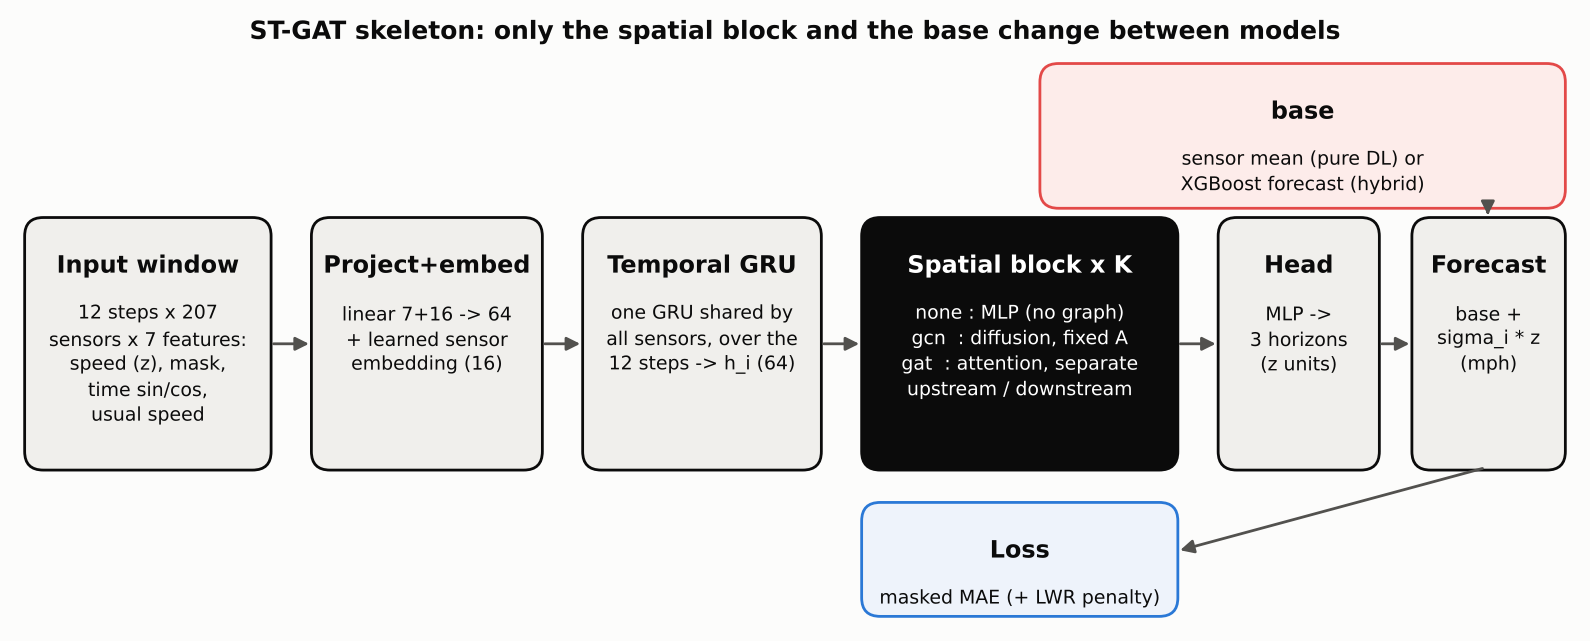
\includegraphics[width=\columnwidth]{fig_dl_architecture}
\caption{Phase~2 skeleton. Only the spatial block changes between the no-graph, diffusion and attention models; the hybrid adds the XGBoost forecast as the base the network corrects.}
\label{fig:arch}
\end{figure}

% ------------------------------------------------------------------------------------
\section{Experimental Setup}
\textbf{Fair comparison.} Same data, masking, split, sample indices, 12-step history, horizons and evaluation code as Phase~1. Phase~1 models are reported from their saved predictions.

\textbf{Training.} AdamW, learning rate $10^{-3}$ ($5\times10^{-4}$ for the hybrid, which starts close to the optimum), batch 64, 8{,}000 random windows per epoch, at most 30 epochs, early stopping with patience 5 on validation masked MAE, best checkpoint restored. Hidden size 64, two graph layers, dropout 0.1. These values were fixed after a short pilot on the validation weeks; the test weeks were scored once, at the end. Everything runs on two CPU cores (no GPU): one main model takes about 40 minutes.

\textbf{Ablations.} To fit the CPU budget, design ablations use a shorter, \emph{identical} budget of 12 epochs and are compared with ST-GAT-short, the main model trained under that same budget. Each changes one thing: number of hops (1/2/3), directed vs undirected edges, the road graph vs a random graph with the same out-degrees and weights, masking vs feeding outages as 0~mph, dropout and weight decay on vs off, and the hybrid with vs without a graph. The two key comparisons --- graph vs no graph, attention vs fixed weights --- use the full budget. Three seeds (12-epoch budget) estimate run-to-run spread.

% ------------------------------------------------------------------------------------
\section{Results}\label{sec:results}
\subsection{Main comparison}
Table~\ref{tab:main} and Fig.~\ref{fig:horizon} give test MAE, RMSE and MAPE on the June weeks, on exactly the Phase~1 samples. Four findings stand out.

\emph{(i) Deep sequence modelling alone already helps at longer horizons.} The GRU without any graph is worse than XGBoost-spatial at 15 minutes (\pMaeGRUFifteen{} vs \pMaeXGBsFifteen{}) but better at 30 and 60 minutes (\pMaeGRUSixty{} vs \pMaeXGBsSixty{}), although it sees no neighbour at all. A learned representation of the whole hour (level, slope, missingness, time) extrapolates further than 34 hand-built features.

\emph{(ii) The road graph adds a consistent gain on top.} With identical size and training, adding two graph-attention layers lowers MAE by \pRelGatVsGruFifteen\%, \pRelGatVsGruThirty\% and \pRelGatVsGruSixty\% at 15/30/60 minutes relative to the no-graph GRU; the fixed-weight diffusion model does the same. Against XGBoost-spatial, ST-GAT ties at 15 minutes (DM $p=\pDmPGATFifteen$) and is significantly better at 30 and 60 minutes (\pChgGATThirty\% and \pChgGATSixty\%, both $p<10^{-10}$) --- precisely the horizons at which the Phase~1 one-hop features faded.

\emph{(iii) Learned attention is not better than fixed road weights here.} DCRNN-lite (\pMaeGCNFifteen/\pMaeGCNThirty/\pMaeGCNSixty) and ST-GAT (\pMaeGATFifteen/\pMaeGATThirty/\pMaeGATSixty) are within a few hundredths of a mph, and the fixed-weight model is even slightly (but significantly) better at 30--60 minutes (\S\ref{sec:sig}). On a freeway graph whose links already encode driving distance, the Gaussian kernel is a good prior; attention earns its place through interpretability (\S\ref{sec:att}) rather than accuracy.

\emph{(iv) The hybrid is the best model at every horizon.} XGBoost + ST-GAT residual reaches \pMaeHybFifteen/\pMaeHybThirty/\pMaeHybSixty~mph, \pChgHybFifteen\%, \pChgHybThirty\% and \pChgHybSixty\% against XGBoost-spatial alone (DM statistics \pDmHybFifteen, \pDmHybThirty, \pDmHybSixty; all $p<10^{-10}$). Its biggest edge over the pure graph network is at 15 minutes (\pRelHybVsGatFifteen\%), where the tree model's sharp use of the current reading and the usual speed matters most; at 60 minutes the two converge, because there the correction carries most of the information. Each part does what it is best at: the tree model the per-sensor level and daily cycle, the graph network the propagation. For reference, DCRNN reports 2.77/3.15/3.60~\cite{li2018dcrnn} after 100 GPU epochs on a slightly different split; our CPU-trained hybrid is within 0.03--0.08~mph.

\begin{table*}[t]\centering
\caption{Test-set masked MAE, RMSE (mph) and MAPE (\%) by horizon, 4--27 June 2012, identical samples for all models. P1 = Phase~1 model, P2 = Phase~2. Best MAE in bold.}
\label{tab:main}\footnotesize\setlength{\tabcolsep}{4pt}
\begin{tabular}{llrrrrrrrrr}\hline
 & & \multicolumn{3}{c}{15 min} & \multicolumn{3}{c}{30 min} & \multicolumn{3}{c}{60 min}\\
Model & & MAE & RMSE & MAPE & MAE & RMSE & MAPE & MAE & RMSE & MAPE\\\hline
Historical average & P1 & 4.19 & 7.86 & 13.1 & 4.19 & 7.86 & 13.1 & 4.19 & 7.86 & 13.1\\
Persistence & P1 & 3.49 & 6.38 & 8.6 & 4.18 & 8.00 & 10.8 & 5.33 & 10.27 & 14.4\\
XGBoost + nbrs & P1 & 2.87 & 5.18 & 7.6 & 3.32 & 6.16 & 9.4 & 3.78 & 7.07 & 11.2\\
Random Forest + nbrs & P1 & 2.87 & 5.16 & 7.7 & 3.31 & 6.09 & 9.4 & 3.81 & 7.06 & 11.3\\
\hline
GRU, no graph & P2 & 2.91 & 5.71 & 8.0 & 3.31 & 6.68 & 9.6 & 3.71 & 7.69 & 11.4\\
Diffusion GCN & P2 & 2.88 & 5.51 & 7.7 & 3.24 & 6.41 & 9.1 & \textbf{3.66} & 7.44 & 10.9\\
ST-GAT & P2 & 2.88 & 5.52 & 7.9 & 3.26 & 6.46 & 9.5 & 3.68 & 7.52 & 11.3\\
ST-GAT + LWR & P2 & 2.88 & 5.53 & 7.9 & 3.25 & 6.46 & 9.4 & 3.68 & 7.50 & 11.2\\
Hybrid XGB+ST-GAT & P2 & \textbf{2.80} & 5.20 & 7.4 & \textbf{3.23} & 6.19 & 9.1 & 3.68 & 7.15 & 11.0\\
\hline\end{tabular}\end{table*}


\begin{figure}[t]\centering
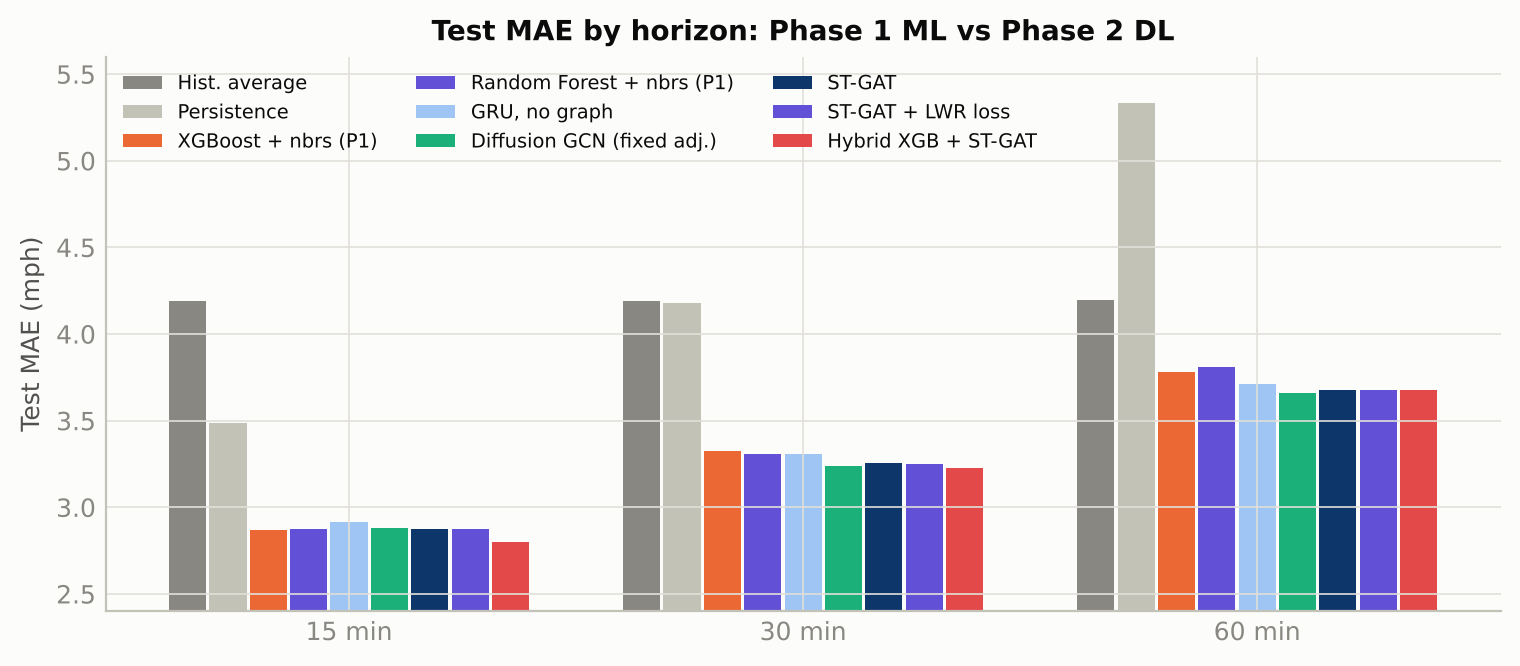
\includegraphics[width=\columnwidth]{fig_dl_mae_by_horizon}
\caption{Test MAE by horizon for the Phase~1 references and the Phase~2 models.}
\label{fig:horizon}
\end{figure}

\subsection{Rush hour}
Table~\ref{tab:peak} and Fig.~\ref{fig:gain} split the 60-minute errors by period. The graph models improve on XGBoost-spatial in both weekday rush hours and off-peak. In mph the gains are similar or slightly larger in the peaks (hybrid: \pPeakXGBsSixty{} $\rightarrow$ \pPeakHybSixty{} peak, \pOffXGBsSixty{} $\rightarrow$ \pOffHybSixty{} off-peak); in relative terms they are slightly larger off-peak (\pChgPeakHybSixty\% vs \pChgOffHybSixty\%), because the off-peak error is small to begin with. The no-graph GRU gains almost nothing in the peaks (\pChgPeakGRUSixty\%) while the diffusion model gains \pChgPeakGCNSixty\%: in rush hour the improvement comes from the graph. Rush hour remains about 1.7$\times$ harder than off-peak for every model; it is still where most of the error is. The congestion map (Fig.~\ref{fig:map}) shows the evening jam of 13~June as forecast an hour ahead.

\begin{table}[t]\centering
\caption{Test MAE (mph) at 60 minutes, weekday rush hours (07--10, 16--19) vs off-peak, and change vs XGBoost-spatial.}
\label{tab:peak}\footnotesize
\begin{tabular}{lrrrr}\hline
Model & Peak & $\Delta$ & Off-peak & $\Delta$\\\hline
XGBoost + nbrs & 5.67 & -- & 3.31 & --\\
GRU, no graph & 5.67 & +0.1\% & 3.22 & -2.7\%\\
Diffusion GCN & 5.54 & -2.2\% & 3.18 & -3.8\%\\
ST-GAT & 5.62 & -0.8\% & 3.19 & -3.6\%\\
ST-GAT + LWR & 5.63 & -0.6\% & 3.18 & -3.7\%\\
Hybrid XGB+ST-GAT & 5.53 & -2.3\% & 3.21 & -3.0\%\\
\hline\end{tabular}\end{table}


\begin{figure*}[t]\centering
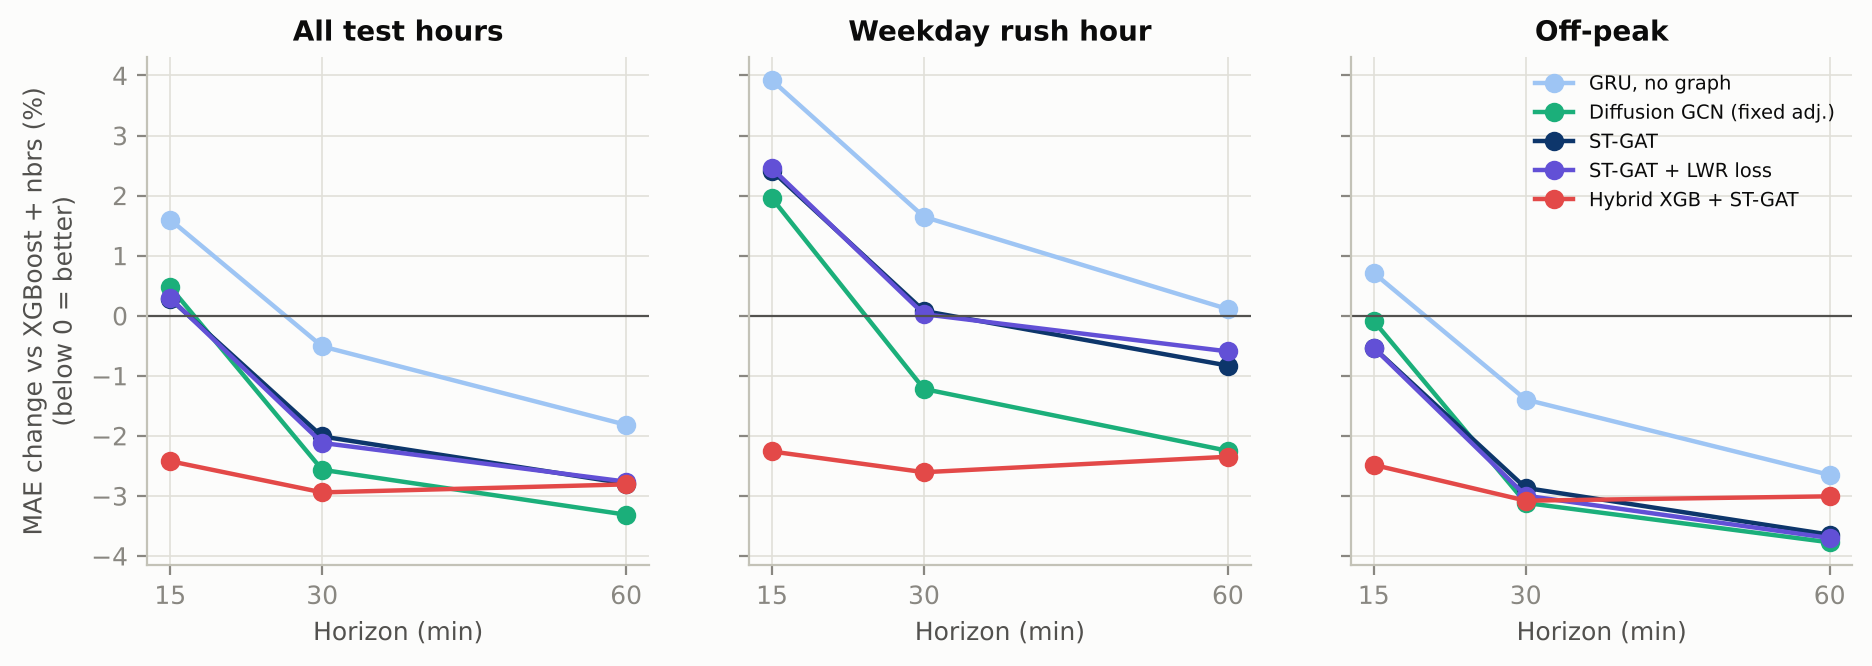
\includegraphics[width=0.95\textwidth]{fig_dl_gain_vs_xgb}
\caption{MAE change of each Phase~2 model relative to XGBoost-spatial (Phase~1's best), overall, in weekday rush hours and off-peak. Below zero is better.}
\label{fig:gain}
\end{figure*}

\begin{figure*}[t]\centering
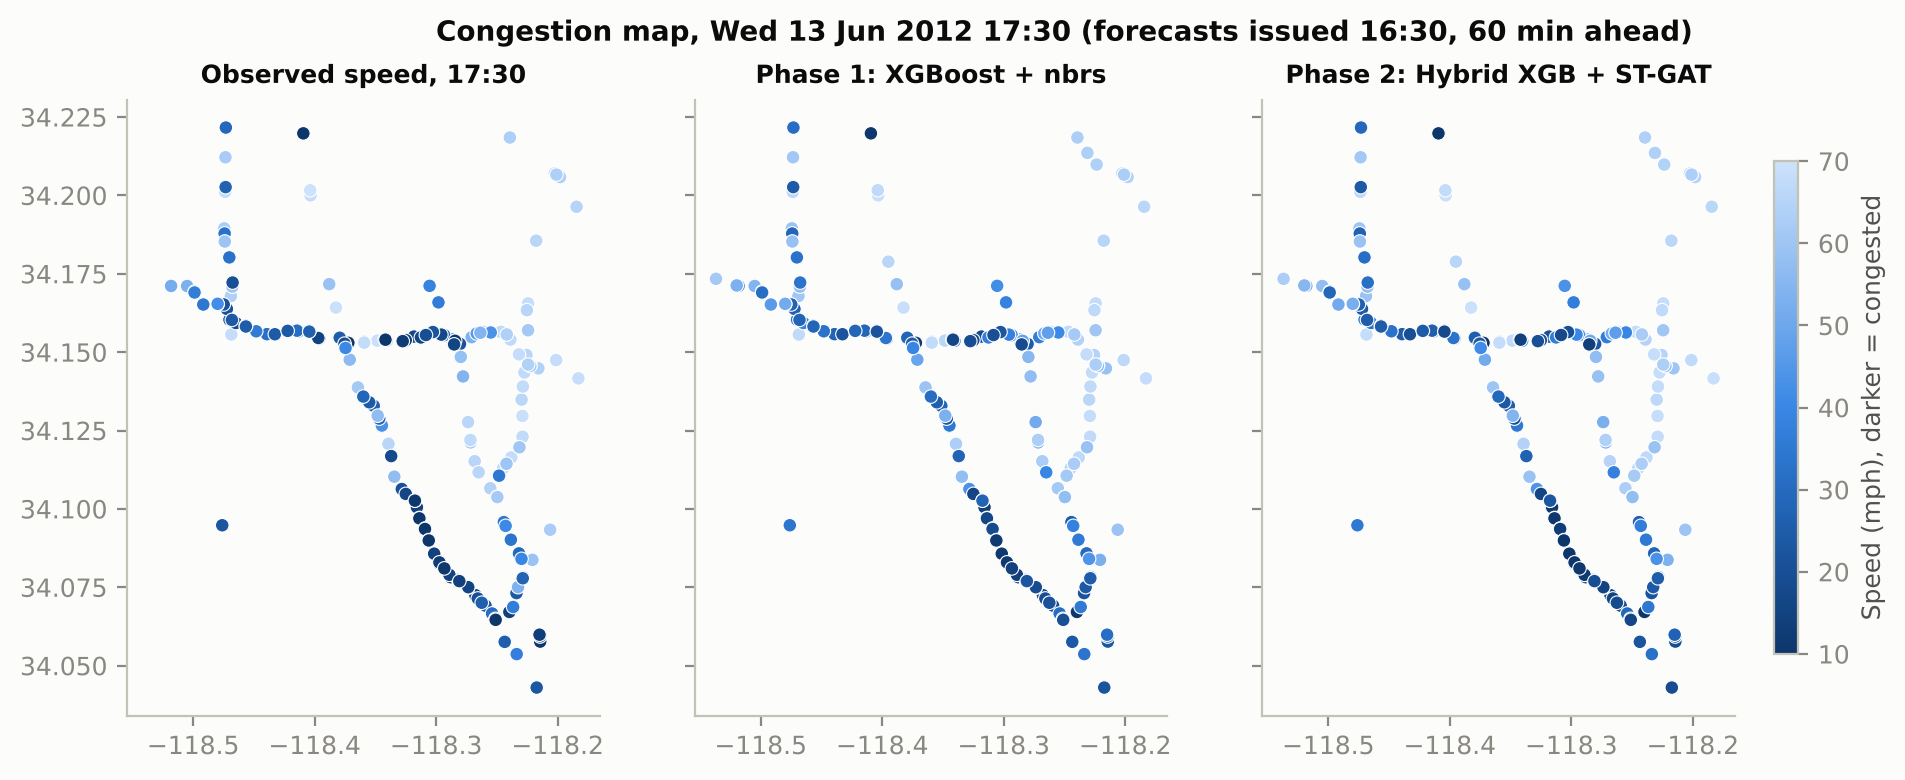
\includegraphics[width=0.95\textwidth]{fig_dl_congestion_map}
\caption{Congestion map, Wednesday 13 June 2012 at 17:30: observed speeds and 60-minute-ahead forecasts from XGBoost-spatial and the best Phase~2 model.}
\label{fig:map}
\end{figure*}

\subsection{Jam detection and large errors}
Scored as a detector of speeds below 35~mph at 60 minutes, the graph models catch more jams than XGBoost-spatial: recall rises from \pRecXGBsSixty{} to \pRecGCNSixty{} (diffusion) and \pRecGATSixty{} (ST-GAT), F1 from \pFoneXGBsSixty{} to \pFoneGCNSixty{} and \pFoneGATSixty, at a small cost in precision. The pure deep models, however, have a \emph{higher RMSE} than XGBoost (\pRmseGATSixty{} vs \pRmseXGBsSixty{} at 60 minutes): trained on absolute error, they predict something close to the conditional median and under-predict the rare, deep speed drops that dominate squared error. The hybrid, anchored on the tree forecast, keeps RMSE close to XGBoost's (\pRmseHybSixty) while improving MAE. A Huber or quantile loss is the natural next step.

\subsection{Is each difference real?}\label{sec:sig}
Table~\ref{tab:dmpairs} applies the Diebold--Mariano test to the key pairs. Adding the graph to the same network is significant at every horizon (ST-GAT vs GRU: DM $=-12.6,-11.4,-4.8$; diffusion vs GRU: $-9.1,-12.4,-6.1$), and so is adding it inside the hybrid (hybrid vs hybrid without graph: $-14.6,-13.2,-11.4$). Attention vs fixed weights goes the other way at 30--60 minutes: the diffusion model is slightly but significantly better ($p<0.01$). The LWR penalty makes no significant difference at any horizon ($p\geq0.09$). The hybrid beats pure ST-GAT at 15 and 30 minutes and ties at 60 ($p=0.96$). These tests treat each trained model as fixed; they do not include run-to-run variation, which we estimate below.

\begin{table}[t]\centering
\caption{Diebold--Mariano statistics for key pairs (negative = first model more accurate), test weeks.}
\label{tab:dmpairs}\footnotesize
\begin{tabular}{lrrr}\hline
Pair & 15 min & 30 min & 60 min\\\hline
ST-GAT vs GRU (no graph) & $-12.6$ & $-11.4$ & $-4.8$\\
Diffusion vs GRU (no graph) & $-9.1$ & $-12.4$ & $-6.1$\\
ST-GAT vs Diffusion & $-2.0$ & $+4.5$ & $+2.8$\\
Hybrid vs hybrid without graph & $-14.6$ & $-13.2$ & $-11.4$\\
Hybrid vs ST-GAT & $-16.4$ & $-4.2$ & $-0.1$\\
ST-GAT+LWR vs ST-GAT & $+0.2$ & $-1.7$ & $+0.3$\\
Hybrid vs XGBoost-spatial & \pDmHybFifteen & \pDmHybThirty & \pDmHybSixty\\
\hline\end{tabular}\end{table}

\subsection{Ablations and seeds}
Table~\ref{tab:abl} and Fig.~\ref{fig:abl} report the design ablations under the identical 12-epoch budget. Three seeds of the reference model give \pSeedMeanFifteen~$\pm$~\pSeedStdFifteen{} mph at 15 minutes and \pSeedMeanSixty~$\pm$~\pSeedStdSixty{} mph at 60 minutes; the reference run (seed 42, \pMaeShortSixty{} at 60 minutes) happens to be the weakest of the three, so differences should be read against this spread. Read that way:
\begin{itemize}
\item \textbf{Hops:} 3 layers reach \pMaeThreeHopSixty{} at 60 minutes, about one seed standard deviation better than 2 layers on average, while 1 layer (\pMaeOneHopSixty) is no better than 2 --- weak evidence, consistent with the LWR argument, that more hops help the longest horizon.
\item \textbf{Graph structure, direction and masking} (random graph \pMaeRandSixty, undirected \pMaeUndirSixty, outages as 0~mph \pMaeZeroSixty{} at 60 minutes) stay within the seed spread under this short budget; the masked model is better at 15 minutes (\pMaeShortFifteen{} vs \pMaeZeroFifteen). Twelve epochs are not enough for the network to exploit the road structure fully; the full-budget, significance-tested comparisons above are the evidence that the graph matters.
\item \textbf{Regularisation:} switching off dropout and weight decay \emph{helps} under the short budget (\pMaeNoDropSixty{} at 60 minutes): with few epochs the model under-fits, and regularisation slows it down further. This is the expected behaviour early in training and is why the main models use early stopping over a longer budget rather than a fixed short one.
\item \textbf{Hybrid without graph} (\pMaeHybNoFifteen/\pMaeHybNoThirty/\pMaeHybNoSixty) is already strong, and the graph version improves on it significantly at every horizon.
\end{itemize}

\begin{table}[t]\centering
\caption{Ablations under an identical 12-epoch budget: test MAE (mph) and change vs the reference ST-GAT-short.}
\label{tab:abl}\footnotesize
\begin{tabular}{lrrrr}\hline
Variant & 15 min & 60 min & $\Delta$15 & $\Delta$60\\\hline
reference (2 hops) & 3.00 & 4.08 & -- & --\\
1 hop & 3.00 & 4.09 & +0.001 & +0.008\\
3 hops & 2.98 & 3.97 & -0.017 & -0.104\\
undirected edges & 2.98 & 4.03 & -0.015 & -0.045\\
random graph & 2.99 & 4.08 & -0.010 & -0.003\\
outages as 0 mph & 3.03 & 4.09 & +0.036 & +0.008\\
no dropout/decay & 2.95 & 3.93 & -0.046 & -0.151\\
hybrid, no graph & 2.81 & 3.70 & -0.191 & -0.381\\
\hline\end{tabular}\end{table}


\begin{figure}[t]\centering
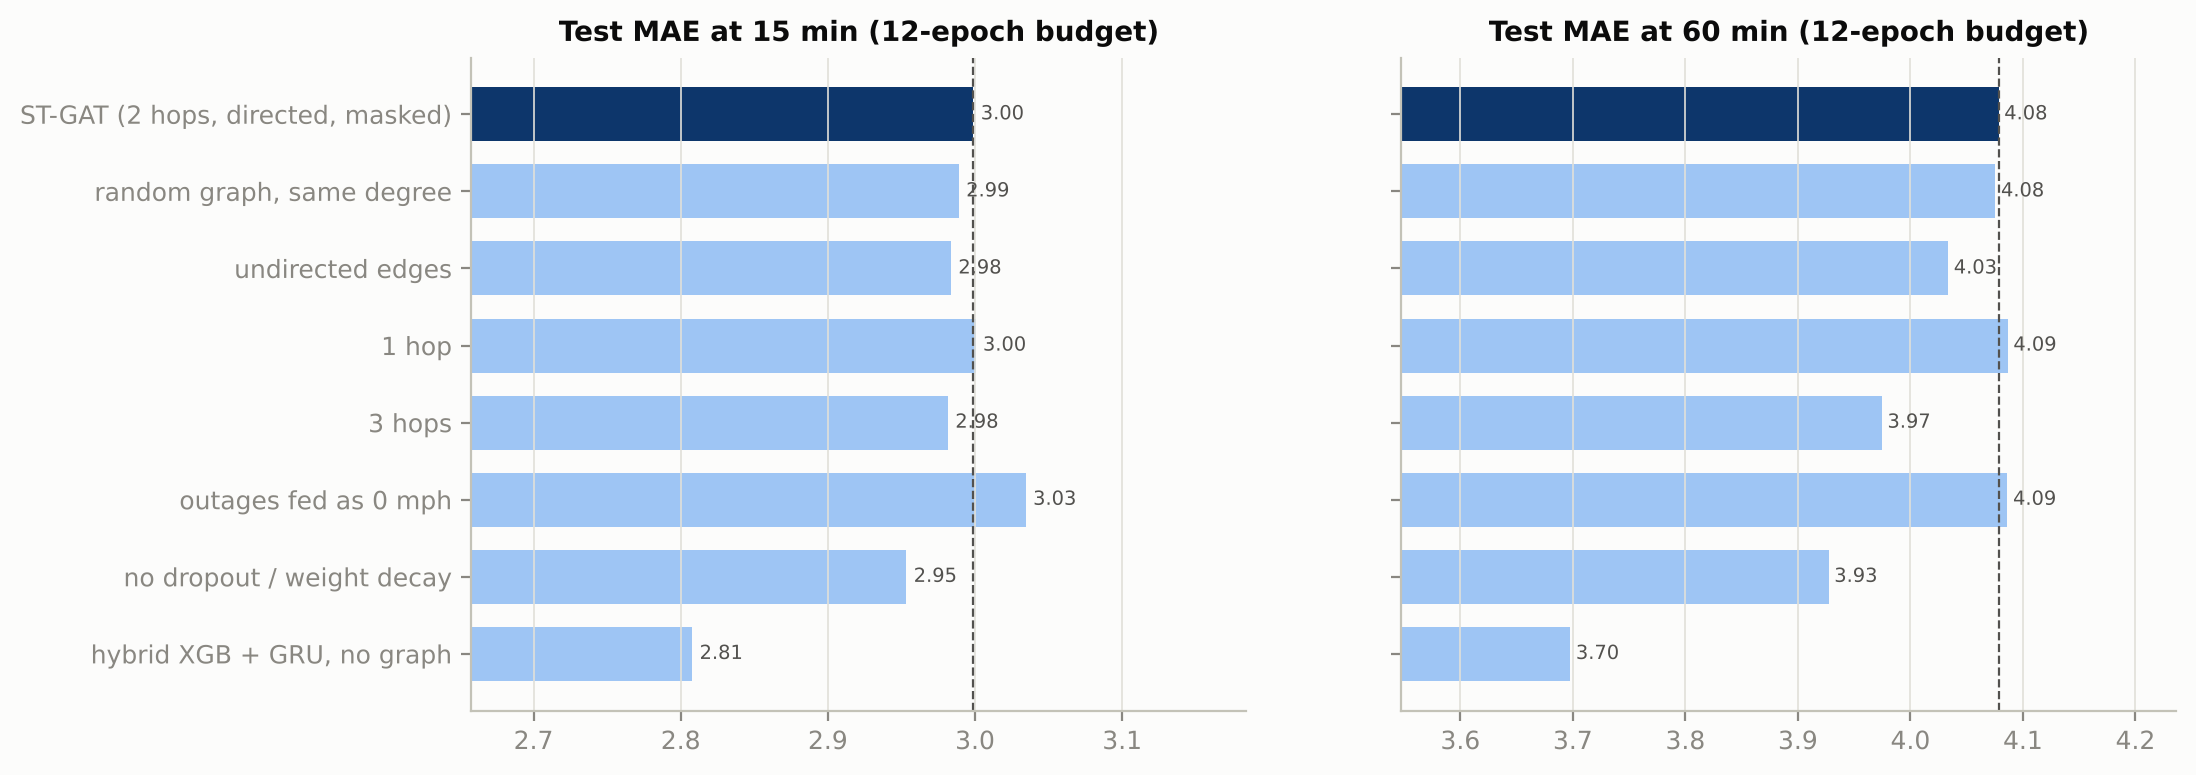
\includegraphics[width=\columnwidth]{fig_dl_ablations}
\caption{Ablations under the same 12-epoch budget; dashed line = reference ST-GAT-short.}
\label{fig:abl}
\end{figure}


\subsection{Where the attention looks}\label{sec:att}
In the undirected ST-GAT one softmax covers a sensor itself and both its upstream and downstream neighbours, so attention shares can be compared (Fig.~\ref{fig:att}). When a sensor is free-flowing it puts \pAttFreeSelf\% of its first-layer attention on itself, \pAttFreeDownstream\% on downstream and \pAttFreeUpstream\% on upstream neighbours; when it is jammed the shares become \pAttJammedSelf\%, \pAttJammedDownstream\% and \pAttJammedUpstream\%. This is an analysis of one trained model and one layer, not a causal statement, but it is the kind of check that relates what the network learned to the LWR picture of queues and platoons.

\begin{figure}[t]\centering
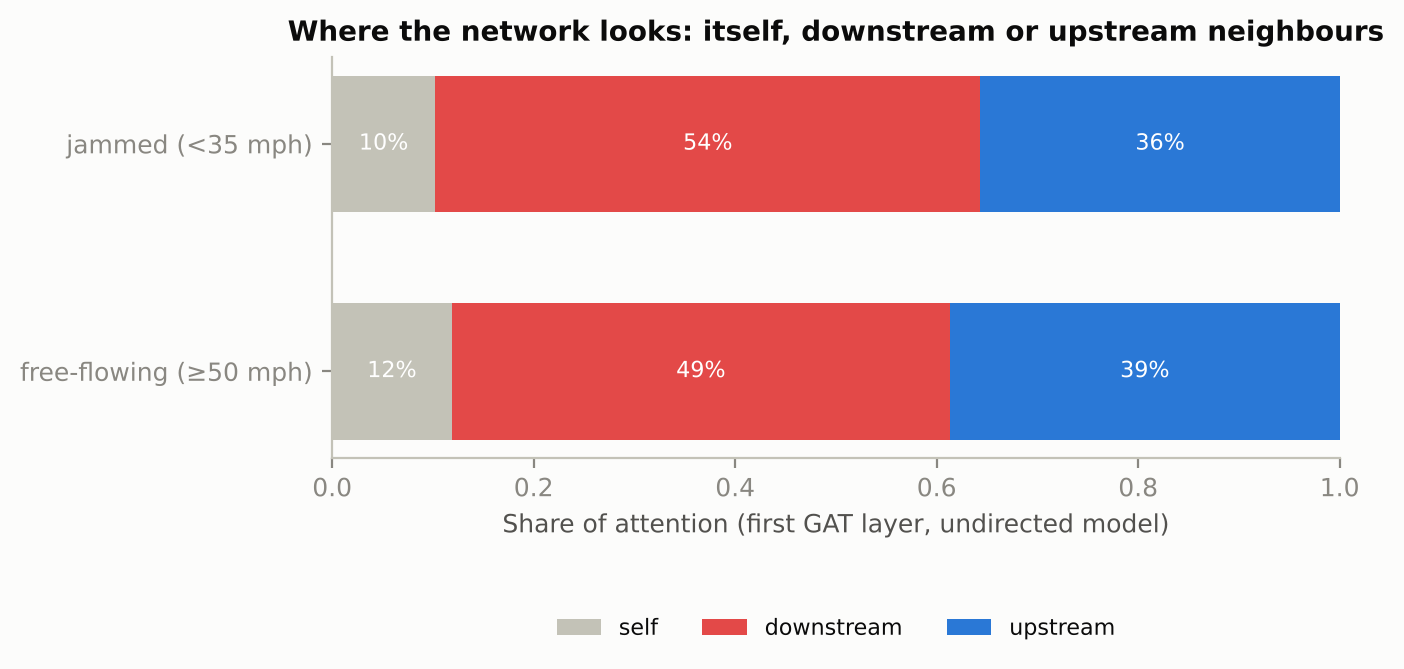
\includegraphics[width=\columnwidth]{fig_dl_attention}
\caption{Share of first-layer attention placed on the sensor itself, its downstream and its upstream neighbours (undirected ST-GAT, 1{,}500 random test times), for free-flowing vs jammed sensors.}
\label{fig:att}
\end{figure}

% ------------------------------------------------------------------------------------
\section{Discussion}
\paragraph{Did Phase 2 close the Phase 1 gap?} Partly, and in the predicted place. Phase~1's one-hop features improved XGBoost by 4.1/3.3/1.8\% at 15/30/60 minutes. Relative to the same deep network without a graph, two layers of message passing improve MAE by \pRelGatVsGruFifteen/\pRelGatVsGruThirty/\pRelGatVsGruSixty\%; relative to XGBoost-spatial the graph models gain most at 30 and 60 minutes and nothing at 15. Information from more than one hop away is useful for the longer horizons, as the LWR picture suggests. The gain is modest --- a few percent --- which is in line with published comparisons between strong single-sensor and graph models once both use the same inputs.

\paragraph{Why the hybrid works} Stacking works when the two models make different mistakes. XGBoost uses the latest reading, the usual speed and the clock very sharply, which makes it hard to beat at 15 minutes; the graph network sees propagation that XGBoost cannot. Learning the residual on \emph{out-of-fold} forecasts is what makes this honest: with in-sample XGBoost predictions the residuals would be close to zero in training and the network would learn nothing useful. The hybrid's edge over the pure graph network is largest at 15 minutes and vanishes at 60, which matches this division of labour.

\paragraph{Attention vs fixed weights; physics} On a freeway graph whose edges come from a distance kernel, the kernel weights are already a sensible guess at who influences whom, so learned attention adds interpretability more than accuracy. The LWR penalty was neutral. Its approximations (Greenshields' diagram, point sensors standing in for road cells, no ramp flows) are coarse, and the data term already pins down the forecast; a stronger physics component would need flow and occupancy data (PeMS) or a learned fundamental diagram.

\paragraph{Limitations} (i)~CPU budget: one run per main model, 30 epochs, 8{,}000 windows per epoch; longer training on a GPU would likely lower every deep model's error. (ii)~Ablations use a 12-epoch budget, so they rank design choices but do not give final accuracies. (iii)~Seed spread was measured on the short budget only. (iv)~The deep models, trained on MAE, have a higher RMSE than XGBoost. (v)~One city and four months of 2012; the test weeks are slightly harder than the training weeks. (vi)~No signal-control experiment was run: the brief makes it optional, and any such result would be a simulation only.

% ------------------------------------------------------------------------------------
\section{Conclusion}
Keeping every element of the Phase~1 protocol fixed, we showed that graph deep learning improves highway-speed forecasts mainly at 30--60 minutes, where one-hop features had faded; that the improvement comes from the graph and not only from deep sequence modelling; that learned attention matches but does not beat fixed road weights on this network; and that a leakage-free hybrid, in which a graph attention network corrects XGBoost, is the best model at every horizon with statistically significant gains. Natural next steps are longer GPU training, a Huber or quantile loss to reduce large misses, PeMS flow and occupancy for a stronger physics term, and a simulated multi-agent signal-control experiment (SUMO or CityFlow~\cite{lopez2018sumo,zheng2019cityflow}) that consumes these forecasts.

% ------------------------------------------------------------------------------------
\section*{Individual Contributions}
\begin{tabular}{@{}p{2.4cm}p{5.3cm}@{}}
\hline
Member & Phase 2 contribution \\
\hline
Kartik Madaan \newline {\footnotesize 2401010212} & DL data pipeline (graph tensors, scaling, mask channel, road-distance matrix), repository, unit tests, reproducibility \\
Arhan Alam \newline {\footnotesize 2401020010} & Architecture: GRU encoder, edge-list graph attention, diffusion block; hop, direction and random-graph ablations \\
Chirag Lalwani \newline {\footnotesize 2401020093} & Training and regularisation (AdamW, dropout, early stopping); out-of-fold XGBoost and the hybrid model \\
Siddhanth Sadshiv Raikar \newline {\footnotesize 2401020110} & DL literature review; LWR physics penalty; report assembly \\
Abhijeet Dey \newline {\footnotesize 2401010014} & Evaluation: horizon/peak metrics, Diebold--Mariano tests, seeds, maps, attention analysis \\
\hline
\end{tabular}
\vspace{2mm}

\noindent All members reviewed every component and can present and defend the full pipeline.


\bibliographystyle{IEEEtran}
\bibliography{refs}

\end{document}
